% !TEX program = xelatex
\documentclass[9pt, aspectratio=169]{beamer}
\usetheme{metropolis}
\usefonttheme{professionalfonts}

% --- Modern Font Setup ---
\usepackage[T1]{fontenc}
\usepackage{FiraSans}  % Modern, elegant sans-serif font family
\usepackage[scaled=0.95]{FiraMono}  % Matching monospace font

% Lighter, more refined font weights
\renewcommand{\seriesdefault}{l}  % Light weight as default
\renewcommand{\bfseries}{\fontseries{sb}\selectfont}  % Semi-bold instead of bold

% Custom font sizing - more refined
\setbeamerfont{title}{size=\Large, series=\fontseries{m}\selectfont}
\setbeamerfont{subtitle}{size=\normalsize, series=\fontseries{l}\selectfont}
\setbeamerfont{author}{size=\small, series=\fontseries{l}\selectfont}
\setbeamerfont{date}{size=\small, series=\fontseries{l}\selectfont}
\setbeamerfont{frametitle}{size=\normalsize, series=\fontseries{m}\selectfont}
\setbeamerfont{framesubtitle}{size=\footnotesize, series=\fontseries{l}\selectfont}
\setbeamerfont{block title}{size=\normalsize, series=\fontseries{m}\selectfont}
\setbeamerfont{block body}{size=\small}
\setbeamerfont{itemize/enumerate body}{size=\small}
\setbeamerfont{itemize/enumerate subbody}{size=\footnotesize}
\setbeamerfont{section in toc}{size=\normalsize, series=\fontseries{m}\selectfont}
\setbeamerfont{section title}{size=\Large, series=\fontseries{m}\selectfont}

% --- Color Definitions ---
% Primary Theme Colors
\definecolor{PrimaryColor}{RGB}{33,52,72}         % Deep navy
\definecolor{SecondaryColor}{RGB}{84,119,146}     % Desaturated blue-gray
\definecolor{AccentColor}{RGB}{100,156,165}       % Soft steel blue
\definecolor{black}{RGB}{0,0,0}
\definecolor{BackgroundColor}{RGB}{245,247,250}   % Very light cool gray/blue-tinted white
\definecolor{TextColor}{RGB}{40,55,70}            % Darker, cool-toned charcoal
\definecolor{LightGray}{RGB}{220,225,230}         % Soft, cool light gray
\definecolor{DarkGray}{RGB}{70,90,105}            % Cool-toned dark gray

% --- Theme Customization ---
\setbeamercolor{background canvas}{bg=BackgroundColor}
\setbeamercolor{normal text}{fg=TextColor}
\setbeamercolor{frametitle}{bg=PrimaryColor, fg=white}
\setbeamercolor{section in toc}{fg=PrimaryColor}
\setbeamercolor{block title}{bg=PrimaryColor!80, fg=white}
\setbeamercolor{block body}{bg=PrimaryColor!10}
\setbeamercolor{alerted text}{fg=AccentColor}
\setbeamercolor{itemize item}{fg=PrimaryColor}
\setbeamercolor{itemize subitem}{fg=SecondaryColor}

% Progress bar
\setbeamercolor{progress bar}{fg=AccentColor, bg=LightGray}

% --- Packages ---
\usepackage[utf8]{inputenc}
\usepackage{url}
\usepackage{booktabs}
\usepackage{amsmath, amssymb, amsfonts}
\usepackage{fontawesome5}
\usepackage{pifont}
\usepackage[most]{tcolorbox}
\tcbuselibrary{skins, listings}
\usepackage{colortbl}
\usepackage{array}
\usepackage{adjustbox}
\usepackage{ragged2e}

% --- Packages for plotting discrete and continuous signals and spectrums ---
\usepackage{tikz}
\usepackage{circuitikz} % Useful for signal processing block diagrams
\usepackage{pgfplots}
\usepackage{graphicx}
\usepackage{caption}
\usepackage{subcaption}

\usetikzlibrary{shapes.callouts, positioning, arrows.meta, shapes.geometric, shadows, calc, patterns, backgrounds, shadings, fit, chains, decorations.pathreplacing, intersections}
\usepgfplotslibrary{fillbetween}
\usepgfplotslibrary{polar}
\pgfplotsset{compat=1.18}
\pgfplotsset{
    plot coordinates/math parser=false,
    signal/.style={thick, color=PrimaryColor},
    spectrum/.style={thick, color=AccentColor},
    discrete/.style={ycomb, mark=*, mark options={fill=white, draw=PrimaryColor}, color=PrimaryColor, thick},
}

% --- Custom Commands ---
\newcommand{\cmark}{\textcolor{PrimaryColor}{\ding{51}}}
\newcommand{\xmark}{\textcolor{AccentColor}{\ding{55}}}
\newcommand{\highlight}[1]{\textcolor{PrimaryColor}{\textbf{#1}}}

% --- Custom tcolorbox environments ---
\newtcolorbox{conceptbox}[1]{
    colback=PrimaryColor!10,
    colframe=PrimaryColor,
    title=#1,
    fonttitle=\small\bfseries,
    fontupper=\small,
    rounded corners
}

\newtcolorbox{insightbox}[1]{
    colback=AccentColor!10,
    colframe=AccentColor,
    title=#1,
    fonttitle=\small\bfseries,
    fontupper=\small,
    rounded corners
}

\newtcolorbox{algorithmbox}[1]{
    colback=SecondaryColor!10,
    colframe=SecondaryColor,
    title=#1,
    fonttitle=\small\bfseries,
    fontupper=\small,
    rounded corners
}

\newtcblisting{codelistingbox}[2][]{
    colback=SecondaryColor!10,
    colframe=SecondaryColor,
    title=#2,
    fonttitle=\small\bfseries,
    rounded corners,
    listing only,
    listing options={
            language=#1,
            basicstyle=\ttfamily\footnotesize,
            keywordstyle=\color{PrimaryColor}\bfseries,
            commentstyle=\color{SecondaryColor}\itshape,
            stringstyle=\color{AccentColor},
            numbers=left,
            numberstyle=\tiny\color{DarkGray},
            stepnumber=1,
            showstringspaces=false,
            tabsize=4
        }
}


\subtitle{Signals and Linear Systems}
\date{}
\author{Ashrafur Rahman\\Lecturer, CSE, BUET}
\institute{ashrafur@cse.buet.ac.bd}


\title{Sampling}

\begin{document}

\maketitle

\begin{frame}{Outline}
    \begin{itemize}
        \item \textbf{Introduction:} Representation of a Continuous-Time Signal by Its Samples
        \item \textbf{Impulse-Train Sampling:} Mathematical Model and Derivation
        \item \textbf{The Sampling Theorem:} Nyquist Rate and Aliasing
        \item \textbf{Signal Reconstruction:}
              \begin{itemize}
                  \item Ideal Low-Pass Filtering
                  \item Zero-Order Hold (ZOH)
                  \item Linear Interpolation
              \end{itemize}
        \item \textbf{Revisiting the DFT:} Practical considerations and periodic signals
    \end{itemize}
\end{frame}

\section{Introduction and Terminology}

\begin{frame}{Recap: Representation by Samples}
    \begin{itemize}
        \item In our review of the DFT, we established that evaluating a continuous-time signal $x(t)$ at uniform intervals $T$ yields a discrete sequence $x[n] = x(nT)$.
        \item \textbf{Question:} Under what conditions can a continuous-time signal be uniquely determined by and exactly recovered from its discrete samples?
        \item This exact recovery is possible if the signal is \textbf{band-limited} (its Fourier Transform is zero outside a finite band of frequencies) and if the samples are taken sufficiently close together.
        \item This fundamental concept is known as the \textbf{Nyquist-Shannon Sampling Theorem}.
    \end{itemize}
\end{frame}

\begin{frame}{Ambiguity in Representation by Samples}
    \begin{itemize}
        \item Generally, infinitely many continuous-time signals can yield the exactly same discrete sequence when sampled at interval $T$.
    \end{itemize}
    \vspace{0.2cm}
    \begin{center}
        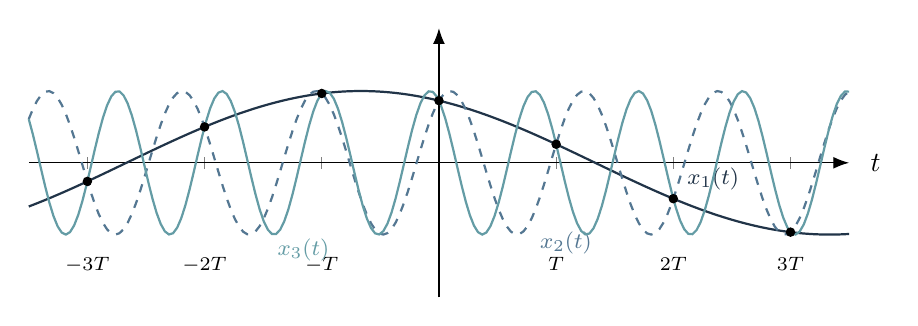
\begin{tikzpicture}
            \begin{axis}[
                width=12cm, height=5cm,
                axis lines=middle, axis line style={-{Latex[length=2mm]}},
                xmin=-3.5, xmax=3.5, ymin=-1.5, ymax=1.5,
                xtick={-3, -2, -1, 1, 2, 3},
                xticklabels={$-3T$, $-2T$, $-T$, $T$, $2T$, $3T$},
                xticklabel style={font=\scriptsize,yshift=-1cm},
                ytick=\empty, xlabel={$t$}, xlabel style={anchor=west, at={(axis cs:3.6,0)}},
                clip=false,
                declare function={
                        x1(\t) = 0.8*cos(deg(pi/4 * \t) + 30);
                        x2(\t) = 0.8*cos(deg(7*pi/4 * \t) - 30);
                        x3(\t) = 0.8*cos(deg(9*pi/4 * \t) + 30);
                    }
                ]
                % Signals
                \addplot[thick, PrimaryColor, domain=-3.5:3.5, samples=200] {x1(x)} node[above right, pos=0.8, font=\footnotesize] {$x_1(t)$};
                \addplot[thick, SecondaryColor, dashed, domain=-3.5:3.5, samples=200] {x2(x)} node[below right, pos=0.6, font=\footnotesize] {$x_2(t)$};
                \addplot[thick, AccentColor, domain=-3.5:3.5, samples=200] {x3(x)} node[below right, pos=0.3, font=\footnotesize] {$x_3(t)$};

                % Sample Points
                \addplot[only marks, mark=*, mark size=1.5pt, black, samples at={-3,-2,-1,0,1,2,3}] {x1(x)};
            \end{axis}
        \end{tikzpicture}
    \end{center}
\end{frame}

\begin{frame}{Impulse-Train Sampling}
    \begin{itemize}
        \item To analyze sampling mathematically, it is convenient to represent the sampling process as multiplying the continuous signal $x(t)$ by a periodic impulse train $p(t)$.
    \end{itemize}

    \begin{conceptbox}{Impulse-Train Modulator}
        \vspace{-0.2cm}
        \begin{equation*}
            p(t) = \sum_{n=-\infty}^{+\infty} \delta(t-nT)
        \end{equation*}
        \begin{equation*}
            x_p(t) = x(t)p(t) = \sum_{n=-\infty}^{+\infty} x(nT)\delta(t-nT)
        \end{equation*}
    \end{conceptbox}

    \begin{center}
        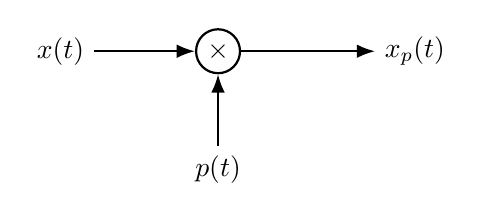
\begin{tikzpicture}[node distance=2cm, auto, >=Latex]
            \node (x) {$x(t)$};
            \node[circle, draw, thick, inner sep=2pt, right of=x] (mult) {$\times$};
            \node[below of=mult, node distance=1.5cm] (p) {$p(t)$};
            \node[right of=mult, node distance=2.5cm] (xp) {$x_p(t)$};

            \draw[->, thick] (x) -- (mult);
            \draw[->, thick] (p) -- (mult);
            \draw[->, thick] (mult) -- (xp);
        \end{tikzpicture}
    \end{center}
\end{frame}

\begin{frame}{Visualizing Impulse-Train Sampling}
    \begin{minipage}{0.48\textwidth}
        \centering
        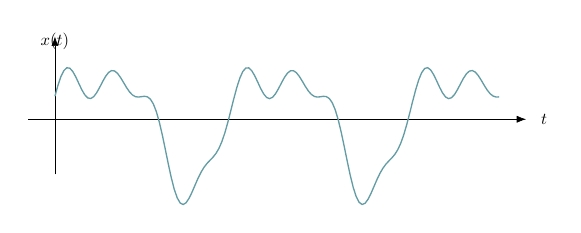
\begin{tikzpicture}[scale=0.6]
            \begin{axis}[
                width=\linewidth, height=4.5cm,
                axis lines=middle, axis line style={-{Latex[length=2mm]}},
                xmin=-0.2, xmax=3.5, ymin=-1.2, ymax=1.8,
                xtick=\empty, ytick=\empty,
                xlabel={$t$}, ylabel={$x(t)$},
                xlabel style={at={(axis cs:3.7,0)}, anchor=east},
                ylabel style={at={(axis cs:0,2.0)}, anchor=north},
                clip=false,
                declare function={sig(\t) = 1.2*sin(deg(1.5*pi*\t)) + 0.5*cos(deg(3*pi*\t)) + 0.3*sin(deg(6*pi*\t));}
                ]
                \addplot[samples=150,domain=0:3.3,thick, AccentColor] {sig(x)};
            \end{axis}
        \end{tikzpicture}
        \vspace{-0.1cm}
        Continuous signal $x(t)$.
    \end{minipage}
    \hfill
    \begin{minipage}{0.48\textwidth}
        \centering
        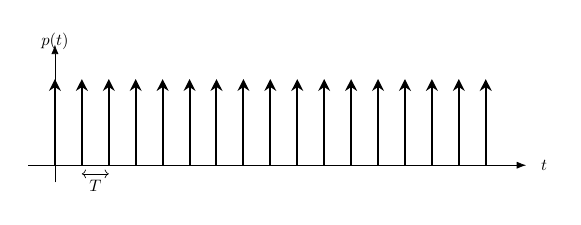
\begin{tikzpicture}[scale=0.6]
            \begin{axis}[
                width=\linewidth, height=4.5cm,
                axis lines=middle, axis line style={-{Latex[length=2mm]}},
                xmin=-0.2, xmax=3.5, ymin=-0.2, ymax=1.4,
                xtick=\empty, ytick=\empty,
                xlabel={$t$}, ylabel={$p(t)$},
                xlabel style={at={(axis cs:3.7,0)}, anchor=east},
                ylabel style={at={(axis cs:0,1.6)}, anchor=north},
                clip=false
                ]
                \addplot[quiver={u=0,v=1}, -{Stealth[length=2.5mm, width=2.5mm]}, very thick, domain=0:3.2, samples=17, color=black] {0};
                \draw[<->] (axis cs:0.2,-0.1) -- node[midway, below] {$T$} (axis cs:0.4,-0.1);
            \end{axis}
        \end{tikzpicture}
        \vspace{-0.1cm}
        Impulse train $p(t)$.
    \end{minipage}

    \vspace{0.4cm}
    \begin{center}
        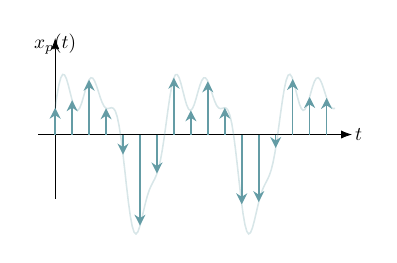
\begin{tikzpicture}[scale=0.7]
            \begin{axis}[
                width=0.6\textwidth, height=4.5cm,
                axis lines=middle, axis line style={-{Latex[length=2mm]}},
                xmin=-0.2, xmax=3.5, ymin=-1.2, ymax=1.8,
                xtick=\empty, ytick=\empty,
                xlabel={$t$}, ylabel={$x_p(t)$},
                xlabel style={at={(axis cs:3.7,0)}, anchor=east},
                ylabel style={at={(axis cs:0,2.0)}, anchor=north},
                clip=false,
                declare function={sig(\t) = 1.2*sin(deg(1.5*pi*\t)) + 0.5*cos(deg(3*pi*\t)) + 0.3*sin(deg(6*pi*\t));}
                ]
                \addplot[samples=150,domain=0:3.3,thick,opacity=0.25, AccentColor] {sig(x)};
                \addplot[quiver={u=0,v=sig(x)}, -{Stealth[length=2mm, width=2mm]}, thick, domain=0:3.2, samples=17, color=AccentColor] {0};
            \end{axis}
        \end{tikzpicture} \\
        Sampled signal $x_p(t)$.
    \end{center}
\end{frame}

\section{Derivation of $X_p(j\omega)$}


\begin{frame}{Fourier Transform and Duality}
    \vspace{-0.2cm}
    \begin{itemize}
        \setbeamertemplate{itemize items}[bullet]
        \item To see the effect of sampling, we need the Fourier Transform of $x_p(t) = x(t)p(t)$.
        \item Let's briefly derive the \textbf{duality principle}. From the inverse Fourier Transform:
              \begin{equation*}
                  x(t) = \frac{1}{2\pi} \int X(j\omega) e^{j\omega t} d\omega \implies 2\pi x(-t) = \int X(j\omega) e^{-j\omega t} d\omega
              \end{equation*}
        \item Swapping $t$ and $\omega$:
              \begin{equation*}
                  2\pi x(-\omega) = \int X(jt) e^{-j\omega t} dt = \mathcal{F}\{X(jt)\}
              \end{equation*}
        \item Hence, the duality principle is as follows:
              \begin{align*}
                  x(t) \stackrel{\mathcal{F}}{\longleftrightarrow} X(j\omega) \implies X(jt) \stackrel{\mathcal{F}}{\longleftrightarrow} 2\pi x(-\omega)
              \end{align*}
    \end{itemize}
\end{frame}

\begin{frame}{Multiplication is Convolution in the Frequency Domain}
    \vspace{-0.2cm}
    \begin{itemize}
        \setbeamertemplate{itemize items}[bullet]
        \item We know from the Convolution Property that,
              \begin{align*}
                  x_1(t) * x_2(t) \stackrel{\mathcal{F}}{\longleftrightarrow} X_1(j\omega)X_2(j\omega)
              \end{align*}
        \item By duality,
              \begin{align*}
                  X_1(jt) * X_2(jt) & \stackrel{\mathcal{F}}{\longleftrightarrow} 2\pi x_1(-\omega)x_2(-\omega) \\
                  X_1(jt)           & \stackrel{\mathcal{F}}{\longleftrightarrow} 2\pi x_1(-\omega)             \\
                  X_2(jt)           & \stackrel{\mathcal{F}}{\longleftrightarrow} 2\pi x_2(-\omega)
              \end{align*}
        \item Substituting $X_1(jt)$ with $u(t)$ and $X_2(jt)$ with $v(t)$:
              \begin{align*}
                  u(t) & \stackrel{\mathcal{F}}{\longleftrightarrow} 2\pi x_1(-\omega)  = U(j\omega) \\
                  v(t) & \stackrel{\mathcal{F}}{\longleftrightarrow} 2\pi x_2(-\omega)  = V(j\omega)
              \end{align*}
        \item Substituting we get:
              \begin{equation*}
                  u(t)v(t) \stackrel{\mathcal{F}}{\longleftrightarrow} \frac{1}{2\pi} U(j\omega) * V(j\omega)
              \end{equation*}
        \item Hence, we can write the Fourier Transform of the sampled signal as:
              \begin{align*}
                  X_p(j\omega) = \frac{1}{2\pi} \left[ X(j\omega) * P(j\omega) \right]
              \end{align*}
    \end{itemize}
\end{frame}

\begin{frame}{Fourier Transform of an Impulse Train}
    \vspace{-0.2cm}
    \begin{itemize}
        \setbeamertemplate{itemize items}[bullet]
        \item Directly taking the Fourier Transform results in a summation that is hard to work with. Instead, we can use the Fourier Series.
        \item $p(t) = \sum_{n=-\infty}^{+\infty} \delta(t-nT)$ is clearly periodic with period $T$ and thus using Fourier Series:
              \begin{equation*}
                  p(t) = \sum_{k=-\infty}^{+\infty} c_k e^{jk\omega_s t}, \quad \text{where } \omega_s = \frac{2\pi}{T}.
              \end{equation*}
        \item Using the \textbf{sifting property} $\int f(t)\delta(t)dt = f(0)$ on period $[-T/2, T/2]$:
              \begin{equation*}
                  c_k = \frac{1}{T} \int_{-T/2}^{T/2} \delta(t) e^{-jk\omega_s t} dt = \frac{1}{T}
              \end{equation*}
        \item Hence, we can write:
              \begin{align*}
                  p(t) = \frac{1}{T} \sum_{k=-\infty}^{+\infty} e^{jk\omega_s t}
              \end{align*}
    \end{itemize}
\end{frame}


\begin{frame}{Fourier Transform of an Impulse Train (cont.)}
    \vspace{-0.2cm}
    \begin{itemize}
        \setbeamertemplate{itemize items}[bullet]

        \item We know the FT of an impulse is 1. By duality, the FT of a constant is an impulse.
              \begin{align*}
                  \delta(t) & \stackrel{\mathcal{F}}{\longleftrightarrow} 1                  \\
                  1         & \stackrel{\mathcal{F}}{\longleftrightarrow} 2\pi\delta(\omega)
              \end{align*}

        \item Using the phase-shifting property:
              \begin{align*}
                  e^{j\omega_0 t} x(t)  \stackrel{\mathcal{F}}{\longleftrightarrow}
                   & \int_{-\infty}^{+\infty} x(t) e^{-j(\omega - \omega_0)t} dt = X(j(\omega - \omega_0))
              \end{align*}
        \item Thus, we have:
              \begin{align*}
                  e^{jk\omega_s t} & \stackrel{\mathcal{F}}{\longleftrightarrow} 2\pi\delta(\omega - k\omega_s)
              \end{align*}
        \item Taking the Continuous-Time Fourier Transform of $p(t)$ term-by-term yields another impulse train:
              \begin{equation*}
                  P(j\omega) =  \frac{1}{T} \sum_{k=-\infty}^{+\infty} \mathcal{F}\{e^{jk\omega_s t}\} = \frac{2\pi}{T} \sum_{k=-\infty}^{+\infty} \delta(\omega - k\omega_s)
              \end{equation*}
    \end{itemize}
\end{frame}

\begin{frame}{Spectrum of the Sampled Signal}
    \begin{itemize}
        \item Now we evaluate the convolution $X_p(j\omega) = \frac{1}{2\pi} X(j\omega) * P(j\omega)$:
              \begin{align*}
                  X_p(j\omega) & = \frac{1}{2\pi} X(j\omega) * \left[ \frac{2\pi}{T} \sum_{k=-\infty}^{+\infty} \delta(\omega - k\omega_s) \right] \\
                               & = \frac{1}{T} \sum_{k=-\infty}^{+\infty} X(j\omega) * \delta(\omega - k\omega_s)
              \end{align*}
        \item For convolution with a shifted impulse, we use the integral definition and sifting property:
              \begin{align*}
                  X(j\omega) * \delta(\omega - \omega_0) & = \int_{-\infty}^{+\infty} X(j\theta)\delta(\omega - \theta - \omega_0) d\theta = X(j(\omega - \omega_0))
              \end{align*}
        \item Thus, we obtain the fundamental equation of sampling:
    \end{itemize}
    \begin{conceptbox}{Spectrum of Sampled Signal}
        \vspace{-0.2cm}
        \begin{equation*}
            X_p(j\omega) = \frac{1}{T} \sum_{k=-\infty}^{+\infty} X(j(\omega - k\omega_s))
        \end{equation*}
    \end{conceptbox}
    \begin{itemize}
        \item $X_p(j\omega)$ consists of periodically repeated copies of $X(j\omega)$, scaled by $1/T$.
    \end{itemize}
\end{frame}

\section{The Sampling Theorem}

\begin{frame}{The Sampling Theorem}
    \begin{itemize}
        \item Suppose $x(t)$ is a \textbf{band-limited} signal, meaning $X(j\omega) = 0$ for $|\omega| > \omega_M$.
        \item The copies of $X(j\omega)$ in $X_p(j\omega)$ are centered at integer multiples of $\omega_s$.
        \item To avoid overlap between adjacent copies, the separation $\omega_s$ must be strictly greater than twice the maximum frequency $\omega_M$.
    \end{itemize}
\end{frame}

\begin{frame}{Nyquist-Shannon Sampling Theorem}
    \vspace{-0.2cm}
    \begin{conceptbox}{Nyquist-Shannon Sampling Theorem}
        Let $x(t)$ be a band-limited signal with $X(j\omega) = 0$ for $|\omega| > \omega_M$. Then $x(t)$ is uniquely determined by its samples $x(nT)$, $n = 0, \pm1, \pm2, \dots$, if
        \begin{equation*}
            \omega_s > 2\omega_M
        \end{equation*}
        where $\omega_s = 2\pi/T$. The minimum sampling frequency $2\omega_M$ is called the \textbf{Nyquist rate}.
    \end{conceptbox}
    \vspace{-0.1cm}
    \begin{center}
        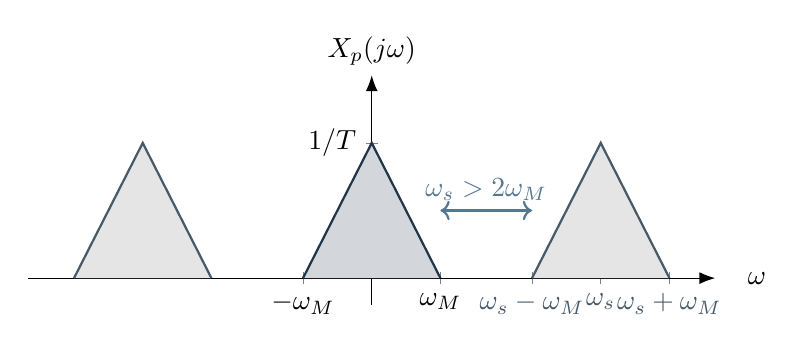
\begin{tikzpicture}
            % Sampled Spectrum X_p(jw)
            \begin{axis}[
                width=0.85\textwidth, height=4.5cm,
                axis lines=middle, axis line style={-{Latex[length=2mm]}},
                xmin=-15, xmax=15, ymin=-0.2, ymax=1.5,
                xtick={-3, 3, 7, 10, 13},
                xticklabels={$-\omega_M$, $\omega_M$, \color{DarkGray}$\omega_s-\omega_M$, \color{DarkGray}$\omega_s$, \color{DarkGray}$\omega_s+\omega_M$},
                ytick={1}, yticklabels={$1/T$},
                xlabel={$\omega$}, ylabel={$X_p(j\omega)$},
                xlabel style={anchor=west, at={(axis cs:16,0)}}, ylabel style={anchor=south},
                clip=false
                ]
                % k=0
                \addplot[thick, PrimaryColor, fill=PrimaryColor!20] coordinates {(-3,0) (0,1) (3,0)};
                % k=1
                \addplot[thick, DarkGray, fill=gray!20] coordinates {(7,0) (10,1) (13,0)};
                % k=-1
                \addplot[thick, DarkGray, fill=gray!20] coordinates {(-13,0) (-10,1) (-7,0)};

                \draw[<->, thick, SecondaryColor] (axis cs:3,0.5) -- node[above] {$\omega_s > 2\omega_M$} (axis cs:7,0.5);
            \end{axis}
        \end{tikzpicture}
    \end{center}
\end{frame}

\begin{frame}{Visualizing the Spectrum: Oversampling}
    \begin{center}
        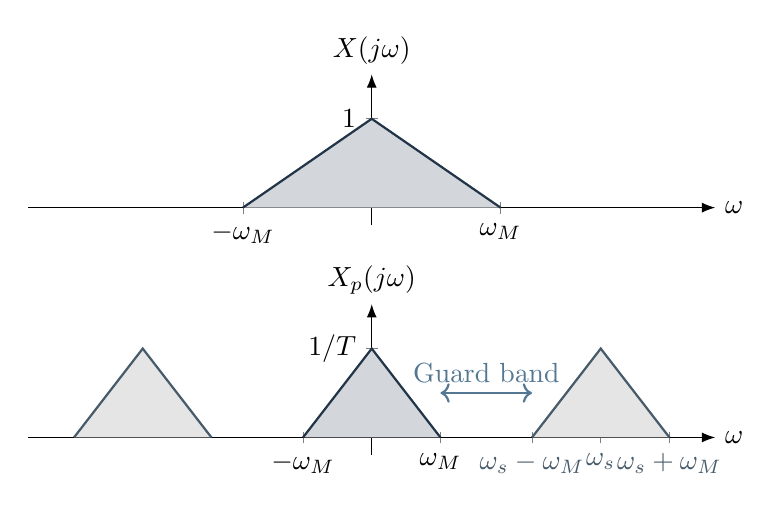
\begin{tikzpicture}
            % Base Spectrum X(jw)
            \begin{axis}[
                name=plot1,
                width=0.85\textwidth, height=3.5cm,
                axis lines=middle, axis line style={-{Latex}},
                xmin=-8, xmax=8, ymin=-0.2, ymax=1.5,
                xtick={-3, 3}, xticklabels={$-\omega_M$, $\omega_M$},
                ytick={1}, yticklabels={$1$},
                xlabel={$\omega$}, ylabel={$X(j\omega)$},
                xlabel style={anchor=west}, ylabel style={anchor=south},
                clip=false
                ]
                \addplot[thick, PrimaryColor, fill=PrimaryColor!20] coordinates {(-3,0) (0,1) (3,0)};
            \end{axis}

            % Sampled Spectrum X_p(jw)
            \begin{axis}[
                name=plot2, at={(plot1.south)}, anchor=north, yshift=-1cm,
                width=0.85\textwidth, height=3.5cm,
                axis lines=middle, axis line style={-{Latex}},
                xmin=-15, xmax=15, ymin=-0.2, ymax=1.5,
                xtick={-3, 3, 7, 10, 13},
                xticklabels={$-\omega_M$, $\omega_M$, \color{DarkGray}$\omega_s-\omega_M$, \color{DarkGray}$\omega_s$, \color{DarkGray}$\omega_s+\omega_M$},
                ytick={1}, yticklabels={$1/T$},
                xlabel={$\omega$}, ylabel={$X_p(j\omega)$},
                xlabel style={anchor=west}, ylabel style={anchor=south},
                clip=false
                ]
                % k=0
                \addplot[thick, PrimaryColor, fill=PrimaryColor!20] coordinates {(-3,0) (0,1) (3,0)};
                % k=1
                \addplot[thick, DarkGray, fill=gray!20] coordinates {(7,0) (10,1) (13,0)};
                % k=-1
                \addplot[thick, DarkGray, fill=gray!20] coordinates {(-13,0) (-10,1) (-7,0)};

                \draw[<->, thick, SecondaryColor] (axis cs:3,0.5) -- node[above] {Guard band} (axis cs:7,0.5);
            \end{axis}
        \end{tikzpicture}
    \end{center}
    \begin{itemize}
        \item When $\omega_s > 2\omega_M$, exact copies of the original spectrum are perfectly separated.
        \item The original signal can be recovered by isolating the baseband copy using a low-pass filter!
    \end{itemize}
\end{frame}

\begin{frame}{Visualizing the Spectrum: Undersampling (Aliasing)}
    \begin{center}
        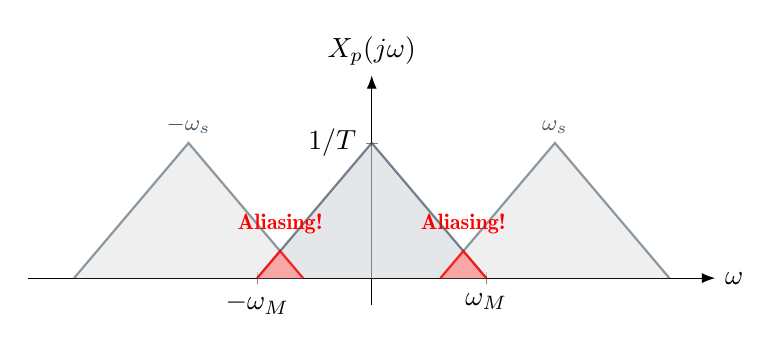
\begin{tikzpicture}
            % Sampled Spectrum X_p(jw) Undersampled
            \begin{axis}[
                width=0.85\textwidth, height=4.5cm,
                axis lines=middle, axis line style={-{Latex}},
                xmin=-15, xmax=15, ymin=-0.2, ymax=1.5,
                xtick={-5, 5},
                xticklabels={$-\omega_M$, $\omega_M$},
                ytick={1}, yticklabels={$1/T$},
                xlabel={$\omega$}, ylabel={$X_p(j\omega)$},
                xlabel style={anchor=west}, ylabel style={anchor=south},
                clip=false
                ]

                % k=1
                \addplot[thick, DarkGray, opacity=0.6, fill=gray!20] coordinates {(3,0) (8,1) (13,0)};
                % k=-1
                \addplot[thick, DarkGray, opacity=0.6, fill=gray!20] coordinates {(-13,0) (-8,1) (-3,0)};
                % k=0
                \addplot[thick, PrimaryColor, opacity=0.6, fill=PrimaryColor!20] coordinates {(-5,0) (0,1) (5,0)};

                % Overlap regions
                \addplot[thick, red, fill=red!40, opacity=0.8] coordinates {(3,0) (4,0.2) (5,0)};
                \addplot[thick, red, fill=red!40, opacity=0.8] coordinates {(-5,0) (-4,0.2) (-3,0)};

                \node[red, font=\footnotesize\bfseries, align=center] at (axis cs: 4, 0.4) {Aliasing!};
                \node[red, font=\footnotesize\bfseries, align=center] at (axis cs: -4, 0.4) {Aliasing!};

                \node[font=\footnotesize, DarkGray, anchor=south] at (axis cs: 8, 1) {$\omega_s$};
                \node[font=\footnotesize, DarkGray, anchor=south] at (axis cs: -8, 1) {$-\omega_s$};
            \end{axis}
        \end{tikzpicture}
    \end{center}
    \begin{itemize}
        \item When $\omega_s < 2\omega_M$, the shifted copies overlap with the baseband spectrum.
        \item High frequencies fold over into the low-frequency band, distorting the signal. This phenomenon is called \textbf{aliasing}.
        \item The original signal $x(t)$ cannot be recovered by low-pass filtering.
    \end{itemize}
\end{frame}

\section{Signal Reconstruction}

\begin{frame}{Ideal Reconstruction}
    \begin{itemize}
        \item By the sampling theorem, if $\omega_s > 2\omega_M$, the \textbf{baseband spectrum} of $x_p(t)$ (the copy of the spectrum $X(j\omega)$ at the origin)
              is an exact replica of $X(j\omega)$ scaled by $1/T$.

        \item We can recover $x(t)$ by applying an \textbf{ideal low-pass filter} to $x_p(t)$.
    \end{itemize}
    \begin{center}
        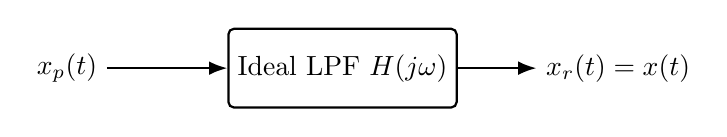
\begin{tikzpicture}[node distance=2.5cm, auto, >=Latex]
            \node (xp) {$x_p(t)$};
            \node[rectangle, draw, thick, rounded corners=2pt, minimum height=1cm, right of=xp, node distance=3.5cm] (filter) {Ideal LPF $H(j\omega)$};
            \node[right of=filter, node distance=3.5cm] (xr) {$x_r(t) = x(t)$};

            \draw[->, thick] (xp) -- (filter);
            \draw[->, thick] (filter) -- (xr);
        \end{tikzpicture}
    \end{center}
    \begin{itemize}
        \item The frequency response of the ideal LPF must be:
              \begin{equation*}
                  H(j\omega) = \begin{cases}
                      T & |\omega| < \omega_c \\
                      0 & |\omega| > \omega_c
                  \end{cases} \quad \text{where} \quad \omega_M < \omega_c < \omega_s - \omega_M
              \end{equation*}
        \item Commonly, we choose the cutoff frequency exactly in the middle: $\omega_c = \omega_s/2$, because it follows the assumption that $\omega_M < \omega_s/2$.
    \end{itemize}
\end{frame}

\begin{frame}{The Ideal Low-Pass Filter}
    \begin{minipage}{0.48\textwidth}
        \centering
        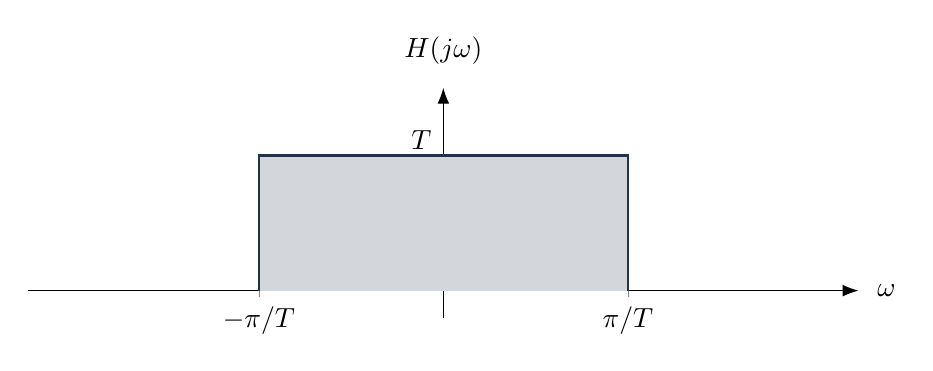
\begin{tikzpicture}
            \begin{axis}[
                width=\textwidth, height=4.5cm,
                axis lines=middle, axis line style={-{Latex[length=2mm]}},
                xmin=-4.5, xmax=4.5, ymin=-0.2, ymax=1.5,
                xtick={-2, 2}, xticklabels={$-\pi/T$, $\pi/T$},
                ytick={1}, yticklabels={$T$},
                yticklabel style={anchor=south east, inner sep=2pt},
                xlabel={$\omega$}, ylabel={$H(j\omega)$},
                xlabel style={anchor=west, at={(axis cs:4.6,0)}},
                ylabel style={anchor=south, at={(axis cs:0,1.6)}},
                clip=false
                ]
                \addplot[thick, PrimaryColor, fill=PrimaryColor!20] coordinates {(-2,0) (-2,1) (2,1) (2,0)};
            \end{axis}
        \end{tikzpicture}
        \vspace{0.1cm}\\
        Frequency Response $H(j\omega)$
    \end{minipage}
    \hfill
    \begin{minipage}{0.48\textwidth}
        \centering
        \begin{tikzpicture}
            \begin{axis}[
                width=\textwidth, height=4.5cm,
                axis lines=middle, axis line style={-{Latex[length=2mm]}},
                xmin=-4.8, xmax=4.8, ymin=-0.4, ymax=1.3,
                xtick={-3,-2,-1,1,2,3}, xticklabels={$-3T$,$-2T$,$-T$,$T$,$2T$,$3T$},
                xticklabel style={font=\footnotesize, yshift=-0.2cm},
                ytick={1}, yticklabels={$1$},
                yticklabel style={anchor=east, xshift=-0.05cm},
                xlabel={$t$}, ylabel={$h(t)$},
                xlabel style={anchor=west, at={(axis cs:5.0,0)}},
                ylabel style={anchor=south, at={(axis cs:0,1.4)}},
                clip=false,
                declare function={
                        sinc(\x) = abs(\x) < 0.001 ? 1 : sin(deg(pi*\x))/(pi*\x);
                    }
                ]
                \addplot[thick, SecondaryColor, domain=-4.5:4.5, samples=150] {sinc(x)};
            \end{axis}
        \end{tikzpicture}
        \vspace{0.1cm}\\
        Impulse Response $h(t)$
    \end{minipage}

    \vspace{0.4cm}
    \begin{itemize}
        \item The frequency response $H(j\omega)$ is a rectangular pulse with cutoff $\omega_c = \omega_s/2 = 2\pi f_s/2 = \pi/T$.
        \item The time-domain impulse response $h(t) = \text{sinc}(t/T)$ extends infinitely in both directions, making the ideal LPF \textbf{unrealizable}.
    \end{itemize}
\end{frame}

\begin{frame}{Deriving the Ideal Interpolation Filter $h(t)$}
    To find the time-domain impulse response $h(t)$ of an ideal low-pass filter with cutoff $\omega_c = \pi/T$ and constant amplitude $T$, we compute the Inverse Fourier Transform:
    \vspace{-0.2cm}
    \begin{align*}
        h(t) & = \frac{1}{2\pi} \int_{-\infty}^{\infty} H(j\omega) e^{j\omega t} d\omega = \frac{1}{2\pi} \int_{-\pi/T}^{\pi/T} T e^{j\omega t} d\omega                                \\
             & = \frac{T}{2\pi} \left[ \frac{e^{j\omega t}}{jt} \right]_{-\pi/T}^{\pi/T} = \frac{T}{\pi t} \left( \frac{e^{j(\pi/T)t} - e^{-j(\pi/T)t}}{2j} \right)                    \\
             & = \frac{T}{\pi t} \sin\left(\frac{\pi t}{T}\right) = \text{sinc}\left(\frac{t}{T}\right) \qquad \left[\text{Recall } \text{sinc}(x) = \frac{\sin(\pi x)}{\pi x} \right]
    \end{align*}
    \medskip

    \textbf{Result:} The time-domain filter corresponding to a perfect frequency cutoff is exactly the infinitely wide $\text{sinc}$ function!
\end{frame}

\begin{frame}{Interpolation with the Ideal LPF}
    \begin{columns}[T]
        \begin{column}{0.55\textwidth}
            \begin{itemize}
                \setbeamertemplate{itemize items}[bullet]
                \item The impulse response $h(t)$ of the ideal LPF (cutoff $\omega_c = \pi/T$) is:
                      \begin{equation*}
                          h(t) = \text{sinc}\left(\frac{t}{T}\right) = \frac{\sin(\pi t/T)}{\pi t/T}
                      \end{equation*}
                \item The reconstructed signal $x_r(t) = x_p(t) * h(t)$ becomes:
                      \begin{align*}
                          x_r(t) & = \left( \sum_{n=-\infty}^{+\infty} x(nT)\delta(t-nT) \right) * h(t)      \\
                                 & = \sum_{n=-\infty}^{+\infty} x(nT) \text{sinc}\left(\frac{t-nT}{T}\right)
                      \end{align*}
                \item Superposition of shifted sinc functions.
            \end{itemize}
        \end{column}
        \begin{column}{0.45\textwidth}
            \vspace{0.2cm}
            \begin{center}
                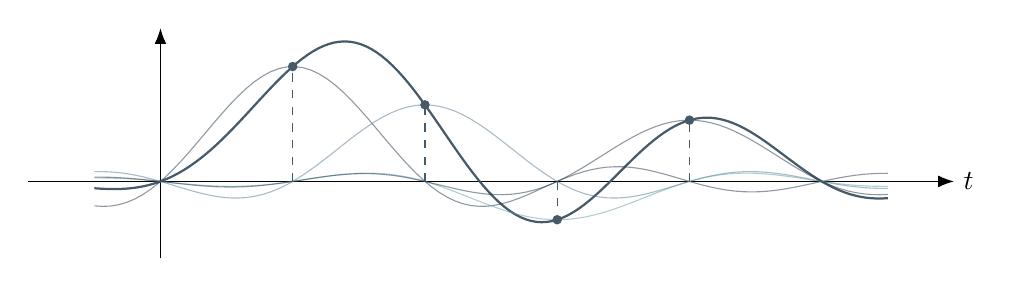
\begin{tikzpicture}
                    \begin{axis}[
                        width=1.1\textwidth, height=4.5cm,
                        axis lines=middle, axis line style={-{Latex[length=2mm]}},
                        xmin=-1, xmax=6, ymin=-1, ymax=2,
                        xtick=\empty, ytick=\empty, xlabel={$t$}, xlabel style={anchor=west, at={(axis cs:6,0)}},
                        clip=false,
                        declare function={
                                sinc(\x) = abs(\x) < 0.001 ? 1 : sin(deg(pi*\x))/(pi*\x);
                                sample(\n) = \n==1 ? 1.5 : (\n==2 ? 1.0 : (\n==3 ? -0.5 : (\n==4 ? 0.8 : 0)));
                            }
                        ]
                        % Total reconstructed signal
                        \addplot[thick, DarkGray, domain=-0.5:5.5, samples=150] {sample(1)*sinc(x-1) + sample(2)*sinc(x-2) + sample(3)*sinc(x-3) + sample(4)*sinc(x-4)};

                        % Individual sinc functions
                        \addplot[PrimaryColor, opacity=0.5, domain=-0.5:5.5, samples=100] {sample(1)*sinc(x-1)};
                        \addplot[SecondaryColor, opacity=0.5, domain=-0.5:5.5, samples=100] {sample(2)*sinc(x-2)};
                        \addplot[AccentColor, opacity=0.5, domain=-0.5:5.5, samples=100] {sample(3)*sinc(x-3)};
                        \addplot[PrimaryColor, opacity=0.5, domain=-0.5:5.5, samples=100] {sample(4)*sinc(x-4)};

                        % Samples
                        \addplot[only marks, mark=*, mark size=1.5pt, DarkGray] coordinates {(1,1.5) (2,1.0) (3,-0.5) (4,0.8)};
                        \draw[dashed, DarkGray] (axis cs:1,0) -- (axis cs:1,1.5);
                        \draw[dashed, DarkGray] (axis cs:2,0) -- (axis cs:2,1.0);
                        \draw[dashed, DarkGray] (axis cs:3,0) -- (axis cs:3,-0.5);
                        \draw[dashed, DarkGray] (axis cs:4,0) -- (axis cs:4,0.8);
                    \end{axis}
                \end{tikzpicture}
            \end{center}
        \end{column}
    \end{columns}
    \vspace{0.2cm}
    \begin{itemize}
        \setbeamertemplate{itemize items}[bullet]
        \item \textbf{However}, $h(t)$ is non-causal and decays very slowly. It is \textbf{unrealizable} in practice. We need approximations.
    \end{itemize}
\end{frame}

\begin{frame}{Zero-Order Hold (ZOH)}
    The simplest practical reconstruction method is the \textbf{Zero-Order Hold (ZOH)}.
    \begin{minipage}{0.48\textwidth}
        \begin{itemize}
            \item \textbf{Concept}: Simply hold the sample value constant until the next sample arrives.
            \item This forms a ``staircase'' approximation $x_0(t)$ of the continuous signal.
            \item Widely used in Digital-to-Analog Converters (DACs).
        \end{itemize}
    \end{minipage}
    \hfill
    \begin{minipage}{0.48\textwidth}
        \centering
        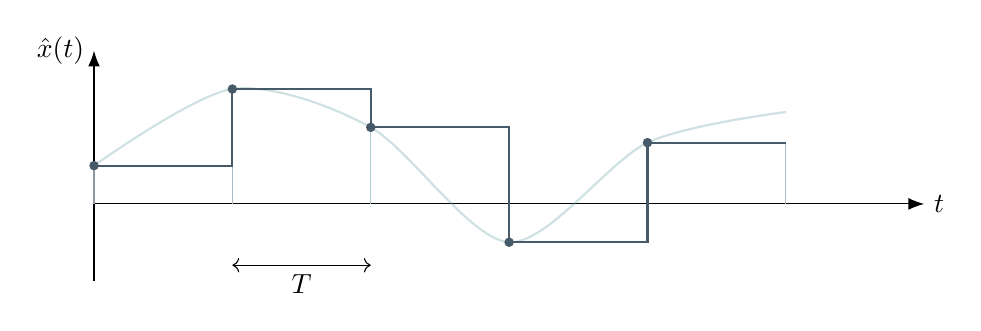
\begin{tikzpicture}
            \begin{axis}[
                width=\textwidth, height=4.5cm,
                axis lines=middle, axis line style={-{Latex[length=2mm]}},
                xmin=0, xmax=6, ymin=-1, ymax=2,
                xtick=\empty, ytick=\empty,
                xlabel={$t$}, ylabel={$\hat{x}(t)$},
                xlabel style={at={(axis cs:6,0)}, anchor=west},
                ylabel style={at={(axis cs:0,2.0)}, anchor=east},
                clip=false
                ]
                % Original continuous signal in background
                \addplot[smooth, thick, opacity=0.3, AccentColor] coordinates {(0,0.5) (1,1.5) (2,1.0) (3,-0.5) (4,0.8) (5,1.2)};

                % Individual ZOH blocks (no fill, thin outlines)
                \addplot[PrimaryColor!50, thin] coordinates {(0,0) (0,0.5) (1,0.5) (1,0)};
                \addplot[SecondaryColor!50, thin] coordinates {(1,0) (1,1.5) (2,1.5) (2,0)};
                \addplot[AccentColor!50, thin] coordinates {(2,0) (2,1.0) (3,1.0) (3,0)};
                \addplot[PrimaryColor!50, thin] coordinates {(3,0) (3,-0.5) (4,-0.5) (4,0)};
                \addplot[SecondaryColor!50, thin] coordinates {(4,0) (4,0.8) (5,0.8) (5,0)};

                % Step sum enveloping the blocks
                \addplot[const plot, thick, DarkGray] coordinates {(0,0.5) (1,1.5) (2,1.0) (3,-0.5) (4,0.8) (5, 0.8)};

                % Original samples
                \addplot[only marks, mark=*, mark size=1.5pt, DarkGray] coordinates {(0,0.5) (1,1.5) (2,1.0) (3,-0.5) (4,0.8)};
                \draw[<->] (axis cs:1,-0.8) -- node[midway, below] {$T$} (axis cs:2,-0.8);
            \end{axis}
        \end{tikzpicture}
    \end{minipage}

    \vspace{0.3cm}
    \begin{itemize}
        \item We can view this mathematically as filtering the impulse-sampled signal $x_p(t)$ with a rectangular pulse $h_0(t)$.
    \end{itemize}
\end{frame}

\begin{frame}{Why is $h_0(t)$ a Rectangle?}
    \begin{itemize}
        \item In a reconstructed output signal, an original sample $y(nT)$ contributes strictly via a shifted, scaled version of the base filter: $y(nT) \cdot h(t - nT)$.
        \item The shape of $h(t)$ dictates the \textbf{weighting} of the sample $y(nT)$ over continuous time.
    \end{itemize}
    \vspace{0.2cm}
    \begin{columns}
        \begin{column}{0.55\textwidth}
            \textbf{For Zero-Order Hold:}
            \begin{itemize}
                \item We desire the sample $y(nT)$ to simply hold its full weight of $1$ constant precisely until the next sample at $(n+1)T$ arrives.
                \item Thus, the isolated weight of $y(nT)$ must jump to $1$ at $t = nT$ and abruptly drop back to $0$ at $t = (n+1)T$.
                \item Therefore, the underlying impulse response $h_0(t)$ \textbf{must} inherently be a rectangular block formally spanning from $0$ to $T$!
            \end{itemize}
        \end{column}
        \begin{column}{0.45\textwidth}
            \centering
            \begin{tikzpicture}
                \begin{axis}[
                    width=\textwidth, height=4.5cm,
                    axis lines=middle, axis line style={-{Latex[length=2mm]}},
                    xmin=-1.0, xmax=2.5, ymin=0, ymax=1.3,
                    ylabel={$y(nT)$},
                    ylabel style={anchor=east},
                    xtick={0.01, 2}, xticklabels={$nT$, $(n+1)T$},
                    ytick={1}, yticklabels={$1$}, clip=false
                    ]
                    \addplot[SecondaryColor, thick] coordinates {(0,1) (2,1)};
                    \draw[dashed, SecondaryColor, thick] (axis cs: 2,1) -- (axis cs: 2,0);
                    \node[SecondaryColor, align=center, font=\footnotesize] at (axis cs: 1, 0.5) {Weight of $y(nT)$\\held at $1$};
                \end{axis}
            \end{tikzpicture}
        \end{column}
    \end{columns}
\end{frame}


\begin{frame}{Deriving the ZOH Frequency Response}
    The ZOH impulse response $h_0(t)$ is simply a rectangular pulse equal to $1$ over $[0, T]$. \\ We construct $H_0(j\omega)$ strictly via continuous Fourier integration:
    \vspace{0.2cm}
    \begin{columns}[T]
        \begin{column}{0.6\textwidth}
            \vspace{-0.4cm}
            \begin{align*}
                H_0(j\omega) & = \int_{-\infty}^{\infty} h_0(t) e^{-j\omega t} dt                                                                        \\
                             & = \int_{0}^{T} (1) e^{-j\omega t} dt = \left[ \frac{e^{-j\omega t}}{-j\omega} \right]_{0}^{T}                             \\
                             & = \frac{1 - e^{-j\omega T}}{j\omega} = \frac{e^{-j\omega T/2} \left( e^{j\omega T/2} - e^{-j\omega T/2} \right)}{j\omega} \\
                             & = e^{-j\omega T/2} \left[ \frac{2}{\omega} \sin\left(\frac{\omega T}{2}\right) \right]                                    \\
                             & = T e^{-j\omega T/2} \, \text{sinc}\left(\frac{\omega T}{2\pi}\right)
            \end{align*}
        \end{column}
        \begin{column}{0.4\textwidth}
            \centering
            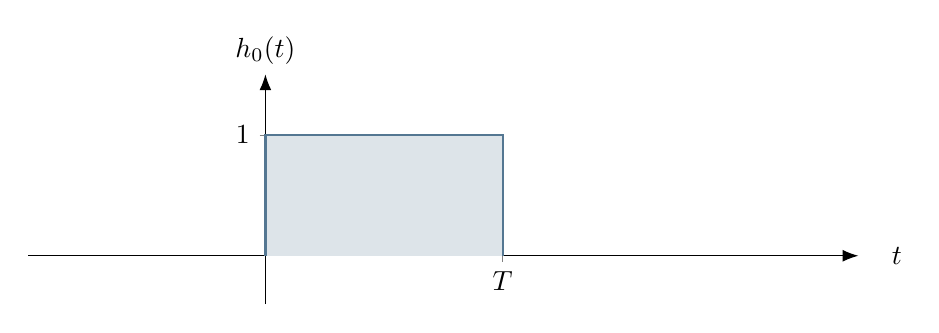
\begin{tikzpicture}
                \begin{axis}[
                    width=\textwidth, height=4.5cm,
                    axis lines=middle, axis line style={-{Latex[length=2mm]}},
                    xmin=-1.0, xmax=2.5, ymin=-0.4, ymax=1.5,
                    xtick={1}, xticklabels={$T$},
                    ytick={1}, yticklabels={$1$},
                    xlabel={$t$}, ylabel={$h_0(t)$},
                    xlabel style={anchor=west, at={(axis cs:2.6,0)}},
                    ylabel style={anchor=south, at={(axis cs:0,1.5)}},
                    clip=false
                    ]
                    \addplot[thick, SecondaryColor, fill=SecondaryColor!20] coordinates {(0,0) (0,1) (1,1) (1,0)};
                \end{axis}
            \end{tikzpicture}
        \end{column}
    \end{columns}
\end{frame}

\begin{frame}{Frequency Domain view of ZOH}
    \begin{minipage}{0.48\textwidth}
        \centering
        \begin{tikzpicture}
            \begin{axis}[
                width=\textwidth, height=4.5cm,
                axis lines=middle, axis line style={-{Latex[length=2mm]}},
                xmin=-8.5, xmax=8.5, ymin=-0.2, ymax=1.5,
                xtick={-4, -2, 2, 4}, xticklabels={$-\omega_s$, \color{PrimaryColor}$-\frac{\omega_s}{2}$, \color{PrimaryColor}$\frac{\omega_s}{2}$, $\omega_s$},
                xticklabel style={font=\footnotesize},
                ytick={1}, yticklabels={$T$},
                yticklabel style={anchor=south east, inner sep=2pt},
                xlabel={$\omega$}, ylabel={$|H_0(j\omega)|$},
                xlabel style={anchor=west, at={(axis cs:8.8,0)}},
                ylabel style={anchor=south, at={(axis cs:0,1.6)}},
                clip=false,
                declare function={
                        zoh(\x) = abs(\x) < 0.001 ? 1 : abs(sin(deg(pi*\x/4))/(pi*\x/4));
                    }
                ]
                % Ideal LPF comparison
                \addplot[PrimaryColor, dashed, thick] coordinates {(-2,0) (-2,1) (2,1) (2,0)};
                \addplot[thick, SecondaryColor, domain=-8.2:8.2, samples=150] {zoh(x)};
            \end{axis}
        \end{tikzpicture}
        \vspace{0.1cm}\\
        Frequency Response $|H_0(j\omega)|$
    \end{minipage}
    \hfill
    \begin{minipage}{0.48\textwidth}
        \centering
        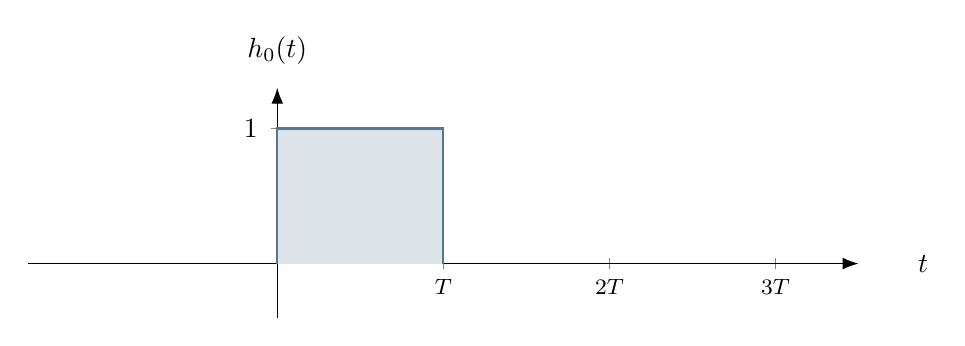
\begin{tikzpicture}
            \begin{axis}[
                width=\textwidth, height=4.5cm,
                axis lines=middle, axis line style={-{Latex[length=2mm]}},
                xmin=-1.5, xmax=3.5, ymin=-0.4, ymax=1.3,
                xtick={1, 2, 3}, xticklabels={$T$, $2T$, $3T$},
                xticklabel style={font=\footnotesize},
                ytick={1}, yticklabels={$1$},
                yticklabel style={anchor=east, xshift=-0.05cm},
                xlabel={$t$}, ylabel={$h_0(t)$},
                xlabel style={anchor=west, at={(axis cs:3.8,0)}},
                ylabel style={anchor=south, at={(axis cs:0,1.4)}},
                clip=false
                ]
                \addplot[thick, SecondaryColor, fill=SecondaryColor!20] coordinates {(0,0) (0,1) (1,1) (1,0)};
            \end{axis}
        \end{tikzpicture}
        \vspace{0.1cm}\\
        Impulse Response $h_0(t)$
    \end{minipage}

    \vspace{0.4cm}
    \begin{itemize}
        \item $h_0(t)$ is a rectangle of width $T$. Its frequency response includes a sinc function: $H_0(j\omega) = T e^{-j\omega T/2} \text{sinc}\left(\frac{\omega T}{2\pi}\right)$.

    \end{itemize}

    We notice that,
    \begin{itemize}
        \item In the passband $|\omega| \le \omega_s/2$, the gain is not constant, attenuating high frequencies slightly.
        \item Outside the passband, the gain is non-zero, allowing high-frequency aliasing copies to leak through.
    \end{itemize}
\end{frame}


\begin{frame}{Linear Interpolation (First-Order Hold)}
    \begin{minipage}{0.48\textwidth}
        \begin{itemize}
            \item \textbf{Linear Interpolation} connects adjacent samples with straight lines.
            \item This produces a continuous, much smoother approximation $x_1(t)$ than the ZOH staircase.
            \item Achieved by filtering the impulse-sampled signal $x_p(t)$ with a triangular pulse $h_1(t)$.
        \end{itemize}
    \end{minipage}
    \hfill
    \begin{minipage}{0.48\textwidth}
        \centering
        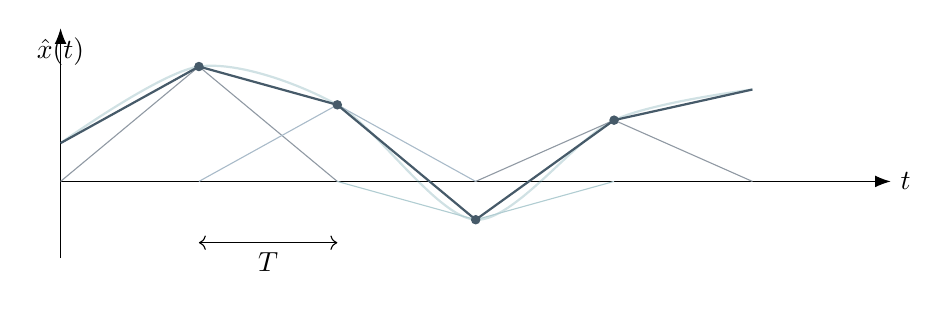
\begin{tikzpicture}
            \begin{axis}[
                width=\textwidth, height=4.5cm,
                axis lines=middle, axis line style={-{Latex[length=2mm]}},
                xmin=0, xmax=6, ymin=-1, ymax=2,
                xtick=\empty, ytick=\empty,
                xlabel={$t$}, ylabel={$\hat{x}(t)$},
                xlabel style={at={(axis cs:6,0)}, anchor=west},
                ylabel style={at={(axis cs:0,2.0)}, anchor=north},
                clip=false
                ]
                % Original continuous signal in background
                \addplot[smooth, thick, opacity=0.3, AccentColor] coordinates {(0,0.5) (1,1.5) (2,1.0) (3,-0.5) (4,0.8) (5,1.2)};

                % Individual FOH triangles (no fill, thin outlines)
                \addplot[PrimaryColor!50, thin] coordinates {(0,0) (1,1.5) (2,0)};
                \addplot[SecondaryColor!50, thin] coordinates {(1,0) (2,1.0) (3,0)};
                \addplot[AccentColor!50, thin] coordinates {(2,0) (3,-0.5) (4,0)};
                \addplot[PrimaryColor!50, thin] coordinates {(3,0) (4,0.8) (5,0)};

                % Linear interpolation enveloping the blocks
                \addplot[thick, DarkGray] coordinates {(0,0.5) (1,1.5) (2,1.0) (3,-0.5) (4,0.8) (5,1.2)};

                % Original samples
                \addplot[only marks, mark=*, mark size=1.5pt, DarkGray] coordinates {(1,1.5) (2,1.0) (3,-0.5) (4,0.8)};
                \draw[<->] (axis cs:1,-0.8) -- node[midway, below] {$T$} (axis cs:2,-0.8);
            \end{axis}
        \end{tikzpicture}
    \end{minipage}

    \vspace{0.3cm}
    \begin{itemize}
        \item The impulse response $h_1(t)$ is a triangle spanning $[-T, T]$ with peak height $1$ at $t=0$.
    \end{itemize}
\end{frame}

\begin{frame}{Why is $h_1(t)$ a Triangle?}
    \begin{itemize}
        \item In a reconstructed signal, a given sample $y(nT)$ contributes via $y(nT) \cdot h_1(t - nT)$.
        \item The shape of $h_1(t)$ thus dictates the \textbf{weighting} of $y(nT)$ over time.
    \end{itemize}
    \vspace{0.2cm}
    \begin{columns}
        \begin{column}{0.5\textwidth}
            \footnotesize

            \textbf{For Linear Interpolation:}

            Given a weight $\alpha \in [0, 1]$, we should have,
            \begin{align*}
                y(t) & = (1 - \alpha) y((n-1)T) + \alpha y(nT) \quad \text{for } t \in [(n-1)T, nT] \\
                y(t) & = (1 - \alpha) y(nT) + \alpha y((n+1)T) \quad \text{for } t \in [nT, (n+1)T]
            \end{align*}
            Therefore,
            \begin{itemize}
                \item The weight of $y(nT)$ should linearly \textit{rise} strictly from $0$ to $1$ between $(n-1)T$ and $nT$.
                \item It should linearly \textit{fall} from $1$ back to $0$ between $nT$ and $(n+1)T$.
                \item At all other times, its weight must precisely be $0$ to isolate its exact local influence.
                \item Therefore, $h_1(t)$ \textbf{must} inherently be a symmetric triangle!
            \end{itemize}
        \end{column}
        \begin{column}{0.5\textwidth}
            \centering
            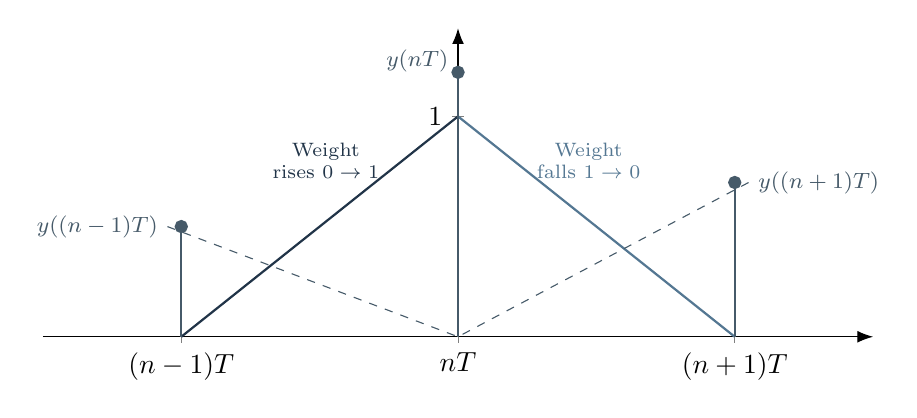
\begin{tikzpicture}
                \begin{axis}[
                    width=\textwidth, height=5.5cm,
                    axis lines=middle, axis line style={-{Latex[length=2mm]}},
                    xmin=-1.5, xmax=1.5, ymin=0, ymax=1.4,
                    xtick={-1, 1}, xticklabels={$(n-1)T$, $(n+1)T$},
                    extra x ticks={0}, extra x tick labels={$nT$},
                    ytick={1}, yticklabels={$1$}, clip=false
                    ]
                    \addplot[PrimaryColor, thick] coordinates {(-1,0) (0,1)};
                    \node[PrimaryColor, align=center, font=\scriptsize, anchor=east] at (axis cs: -0.25, 0.8) {Weight\\rises $0\to 1$};

                    \addplot[SecondaryColor, thick] coordinates {(0,1) (1,0)};
                    \node[SecondaryColor, align=center, font=\scriptsize, anchor=west] at (axis cs: 0.25, 0.8) {Weight\\falls $1\to 0$};

                    \draw[dashed, DarkGray] (axis cs: 0,0) -- (axis cs: 0,1);
                    \draw[dashed, DarkGray] (axis cs: -1.05,0.5) -- (axis cs: 0,0);
                    \draw[dashed, DarkGray] (axis cs: 1.05,0.7) -- (axis cs: 0,0);

                    \addplot[ycomb, mark=*, DarkGray, thick] coordinates {(-1,0.5) (0,1.2) (1,0.7)};
                    \node[DarkGray, anchor=east, font=\footnotesize] at (axis cs: -1.05, 0.5) {$y((n-1)T)$};
                    \node[DarkGray, anchor=east, font=\footnotesize] at (axis cs: 0, 1.25) {$y(nT)$};
                    \node[DarkGray, anchor=west, font=\footnotesize] at (axis cs: 1.05, 0.7) {$y((n+1)T)$};
                \end{axis}
            \end{tikzpicture}
        \end{column}
    \end{columns}
\end{frame}

\begin{frame}{First-Order Hold: Convolution Intuition}
    A linear interpolation triangle filter $h_1(t)$ can be formed by convolving two shifted zero-order hold rectangles!
    \vspace{-0.2cm}
    \begin{equation*}
        h_1(t) = \frac{1}{T} \Big( h_0(t+T/2) * h_0(t+T/2) \Big)
    \end{equation*}
    \vspace{-0.2cm}
    \begin{columns}
        \begin{column}{0.4\textwidth}
            \centering
            \begin{tikzpicture}
                \begin{axis}[
                    name=rectplot, width=\textwidth, height=3.5cm,
                    axis lines=middle, axis line style={-{Latex[length=2mm]}},
                    xmin=-1.5, xmax=1.5, ymin=0, ymax=1.5,
                    xtick={-0.5, 0.5}, xticklabels={$-\frac{T}{2}$, $\frac{T}{2}$},
                    ytick={1}, yticklabels={$1$}, clip=false,
                    yticklabel style={yshift=0.2cm},
                    title={\footnotesize Rectangles overlapping}
                    ]
                    \addplot[PrimaryColor, thick] coordinates {(-0.5,0) (-0.5,1) (0.5,1) (0.5,0)};
                    \addplot[SecondaryColor, thick, dashed] coordinates {(-1.4,0) (-1.4,1) (-0.4,1) (-0.4,0)};
                    \draw[->, thick, SecondaryColor] (axis cs: 0.4, 1.2) -- node[above]{\footnotesize slide} (axis cs: 0.8, 1.2);
                \end{axis}
                \begin{axis}[
                    at={(rectplot.below south west)}, anchor=above north west, yshift=-0.5cm,
                    width=\textwidth, height=3.5cm,
                    axis lines=middle, axis line style={-{Latex[length=2mm]}},
                    xmin=-1.5, xmax=1.5, ymin=0, ymax=1.5,
                    xtick={-1, 1}, xticklabels={$-T$, $T$},
                    ytick={1}, yticklabels={$1$}, ylabel={$h_1(t)$}, clip=false
                    ]
                    \addplot[DarkGray, thick] coordinates {(-1,0) (0,1) (1,0)};
                \end{axis}
            \end{tikzpicture}
        \end{column}
        \begin{column}{0.6\textwidth}
            \begin{itemize}
                \item $h_0(t+T/2)$ is just the standard ZOH block, centered exactly on time $t=0$.
                \item Area of overlap grows linearly to a peak, and drops cleanly linearly!
                \item The peak area is $T \times 1 = T$, hence the factor $\frac{1}{T}$, as the triangle peak should be $1$.
            \end{itemize}
            \vspace{0.4cm}
            \textbf{Frequency Derivation:} Use $\mathcal{F}\{ x * x \} = \mathcal{F}\{x\}^2$.
            \vspace{-0.2cm}
            \begin{align*}
                H_1(j\omega) & = \frac{1}{T} \left[ \mathcal{F}\Big\{ h_0(t+T/2) \Big\} \right]^2             \\
                             & = \frac{1}{T} \left[ T \, \text{sinc}\Big(\frac{\omega T}{2\pi}\Big) \right]^2 \\
                             & = T \, \text{sinc}^2\left(\frac{\omega T}{2\pi}\right)
            \end{align*}
        \end{column}
    \end{columns}
\end{frame}

\begin{frame}{Frequency Domain view of Linear Interpolation}
    \begin{minipage}{0.48\textwidth}
        \centering
        \begin{tikzpicture}
            \begin{axis}[
                width=\textwidth, height=4.5cm,
                axis lines=middle, axis line style={-{Latex[length=2mm]}},
                xmin=-8.5, xmax=8.5, ymin=-0.2, ymax=1.5,
                xtick={-4, -2, 2, 4}, xticklabels={$-\omega_s$, \color{PrimaryColor}$-\frac{\omega_s}{2}$, \color{PrimaryColor}$\frac{\omega_s}{2}$, $\omega_s$},
                xticklabel style={font=\footnotesize},
                ytick={1}, yticklabels={$T$},
                yticklabel style={anchor=south east, inner sep=2pt},
                xlabel={$\omega$}, ylabel={$|H_1(j\omega)|$},
                xlabel style={anchor=west, at={(axis cs:8.8,0)}},
                ylabel style={anchor=south, at={(axis cs:0,1.6)}},
                clip=false,
                declare function={
                        foh(\x) = abs(\x) < 0.001 ? 1 : (sin(deg(pi*\x/4))/(pi*\x/4))^2;
                    }
                ]
                % Ideal LPF comparison
                \addplot[PrimaryColor, dashed, thick] coordinates {(-2,0) (-2,1) (2,1) (2,0)};
                \addplot[thick, DarkGray, domain=-8.2:8.2, samples=150] {foh(x)};
            \end{axis}
        \end{tikzpicture}
        \vspace{0.1cm}\\
        Frequency Response $|H_1(j\omega)|$
    \end{minipage}
    \hfill
    \begin{minipage}{0.48\textwidth}
        \centering
        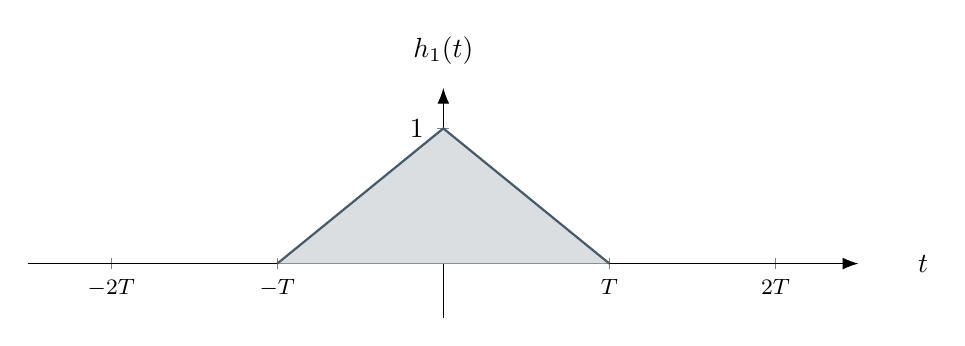
\begin{tikzpicture}
            \begin{axis}[
                width=\textwidth, height=4.5cm,
                axis lines=middle, axis line style={-{Latex[length=2mm]}},
                xmin=-2.5, xmax=2.5, ymin=-0.4, ymax=1.3,
                xtick={-2, -1, 1, 2}, xticklabels={$-2T$, $-T$, $T$, $2T$},
                xticklabel style={font=\footnotesize},
                ytick={1}, yticklabels={$1$},
                yticklabel style={anchor=east, xshift=-0.05cm},
                xlabel={$t$}, ylabel={$h_1(t)$},
                xlabel style={anchor=west, at={(axis cs:2.8,0)}},
                ylabel style={anchor=south, at={(axis cs:0,1.4)}},
                clip=false
                ]
                \addplot[thick, DarkGray, fill=DarkGray!20] coordinates {(-1,0) (0,1) (1,0)};
            \end{axis}
        \end{tikzpicture}
        \vspace{0.1cm}\\
        Impulse Response $h_1(t)$
    \end{minipage}

    \vspace{0.4cm}
    \begin{itemize}
        \item $h_1(t)$ is a triangular pulse spanning $[-T, T]$. Its frequency response is $H_1(j\omega) = T \text{sinc}^2\left(\frac{\omega T}{2\pi}\right)$.
        \item Because of the convolution property, $H_1(j\omega)$ is proportional to the square of the ZOH response, without the phase delay.
    \end{itemize}
\end{frame}

\begin{frame}{Comparing Reconstruction Filters}
    \begin{itemize}
        \item Let's compare the frequency domain magnitudes against the ideal filter (assuming $T=1$):
    \end{itemize}
    \begin{center}
        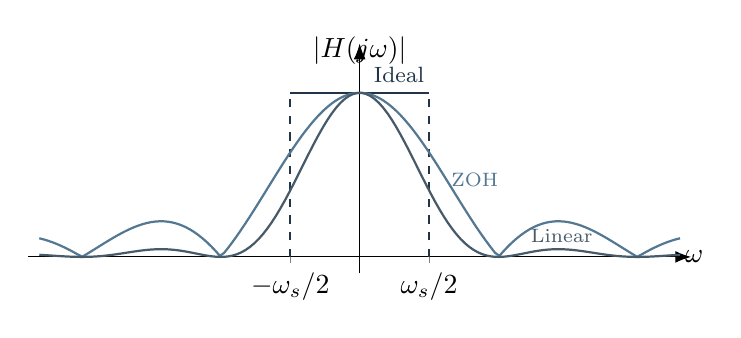
\begin{tikzpicture}
            \begin{axis}[
                width=10cm, height=4.5cm,
                axis lines=middle, axis line style={-{Latex[length=2mm]}},
                xmin=-15, xmax=15, ymin=-0.1, ymax=1.3,
                xtick={-3.14, 3.14}, xticklabels={$-\omega_s/2$, $\omega_s/2$},
                ytick=\empty,
                xlabel={$\omega$}, ylabel={$|H(j\omega)|$},
                xlabel style={at={(axis cs:16,0)}, anchor=east},
                ylabel style={at={(axis cs:0,1.4)}, anchor=north},
                clip=false,
                declare function={
                        zoh(\x)=abs(sin(deg(\x/2))/(\x/2));
                        foh(\x)=zoh(\x)^2;
                    }
                ]
                % Ideal
                \addplot[thick, PrimaryColor, domain=-3.14:3.14, samples=2] {1};
                \draw[thick, PrimaryColor, dashed] (axis cs:-3.14,0) -- (axis cs:-3.14,1);
                \draw[thick, PrimaryColor, dashed] (axis cs:3.14,0) -- (axis cs:3.14,1);

                % ZOH
                \addplot[thick, SecondaryColor, domain=-14.5:14.5, samples=150] {x==0 ? 1 : zoh(x)};

                % FOH
                \addplot[thick, DarkGray, domain=-14.5:14.5, samples=150] {x==0 ? 1 : foh(x)};

                \node[PrimaryColor, font=\footnotesize, anchor=south west] at (axis cs: 0.2, 1) {Ideal};
                \node[SecondaryColor, font=\scriptsize, anchor=west, inner sep=1pt] at (axis cs: 4, 0.47) {ZOH};
                \node[DarkGray, font=\scriptsize, anchor=west, inner sep=1pt] at (axis cs: 7.6, 0.13) {Linear};
            \end{axis}
        \end{tikzpicture}
    \end{center}
    \begin{itemize}
        \item Linear interpolation has much faster high-frequency rolloff (less leakage) than ZOH, making it a "better" low-pass filter approximation.
    \end{itemize}
\end{frame}

\section{Connection to the DFT}

\begin{frame}{Practical Limitation: Time vs. Frequency}
    \begin{columns}
        \begin{column}{0.42\textwidth}
            \begin{insightbox}{The Uncertainty Principle}
                Signals \textbf{cannot} be both time-limited and strictly band-limited!
                \begin{itemize}
                    \item Finite-duration captures mean $X(j\omega)$ inherently extends to infinite frequencies.\footnote{Interesting watch: \href{https://youtu.be/MBnnXbOM5S4}{3Blue1Brown - Uncertainty Principle}}
                \end{itemize}
            \end{insightbox}
            \begin{conceptbox}{Unavoidable Aliasing}
                Sampling \textit{any} real-world signal causes some aliasing! The infinite spectral tails will always overlap and leak into our baseband.
            \end{conceptbox}
        \end{column}

        \begin{column}{0.54\textwidth}
            \vspace*{0.3cm}

            \centering
            \textbf{Time-Limited Signal} \\
            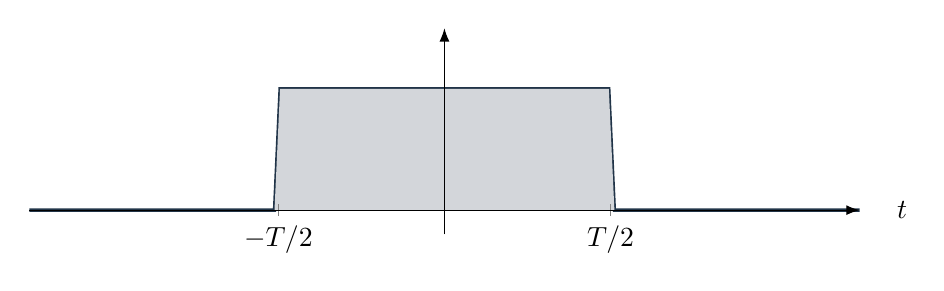
\begin{tikzpicture}
                \begin{axis}[
                    width=\textwidth, height=4.2cm, axis on top,
                    axis lines=middle, axis line style={-{Latex}},
                    xmin=-5, xmax=5, ymin=-0.2, ymax=1.5,
                    xtick={-2, 2}, xticklabels={$-T/2$, $T/2$},
                    ytick=\empty, xlabel={$t$}, clip=false,
                    xlabel style={anchor=west, xshift=10pt},
                    declare function={
                            box(\x) = and(\x>=-2, \x<=2) * 1.0;
                        }
                    ]
                    \addplot[samples=150, domain=-5:5, very thick, PrimaryColor] {box(x)};
                    \addplot[fill=PrimaryColor!20, draw=none, domain=-5:5, samples=150] {box(x)} \closedcycle;
                \end{axis}
            \end{tikzpicture}

            \vspace{0.1cm}
            \textbf{Infinite Frequency Spectrum \& Aliasing} \\ \smallskip
            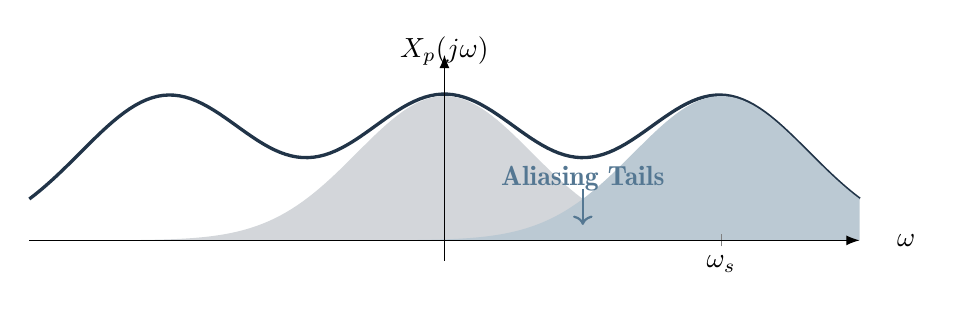
\begin{tikzpicture}
                \begin{axis}[
                    width=\textwidth, height=4.2cm, axis on top,
                    axis lines=middle, axis line style={-{Latex}},
                    xmin=-15, xmax=15, ymin=-0.2, ymax=1.8,
                    xtick={0, 10}, xticklabels={$0$, $\omega_s$},
                    ytick=\empty, xlabel={$\omega$}, ylabel={$X_p(j\omega)$}, clip=false,
                    xlabel style={anchor=west, xshift=10pt}, ylabel style={yshift=10pt, anchor=north},
                    declare function={
                            widegauss(\x) = 1.4*exp(-(\x*\x)/20);
                            dtft(\x) = widegauss(\x) + widegauss(\x-10) + widegauss(\x+10);
                        }
                    ]
                    \addplot[samples=150, domain=-15:15, very thick, PrimaryColor] {dtft(x)};
                    \addplot[fill=PrimaryColor!20, draw=none, domain=-15:15, samples=150] {widegauss(x)} \closedcycle;
                    \addplot[fill=SecondaryColor!40, draw=none, domain=-15:15, samples=150] {widegauss(x-10)} \closedcycle;

                    \node[SecondaryColor, font=\bfseries] at (axis cs:5, 0.6) {Aliasing Tails};
                    \draw[->, thick, SecondaryColor] (axis cs:5, 0.5) -- (axis cs:5, 0.15);
                \end{axis}
            \end{tikzpicture}
        \end{column}
    \end{columns}
\end{frame}

\begin{frame}{The Path to the DFT (Aperiodic Signals)}
    \begin{columns}
        \begin{column}{0.42\textwidth}
            \begin{insightbox}{DTFT}
                The DTFT is exactly the Fourier transform of the impulse train $x_p(t)$ as we saw earlier!
            \end{insightbox}
            \begin{conceptbox}{What does the DFT do?}
                The $N$-point DFT simply grabs $N$ evenly spaced samples of this spectrum from $0$ to $\omega_s$:
                \vspace{-0.2cm}
                \begin{equation*}
                    X[k] = X_p\left(j\frac{k\omega_s}{N}\right)
                \end{equation*}
                {\footnotesize The rightmost bins naturally wrap back negative frequencies!}
            \end{conceptbox}
        \end{column}

        \begin{column}{0.54\textwidth}
            \vspace*{0.3cm}
            \centering
            \textbf{Transform of periodically sampled $x(t)$} \\ \smallskip
            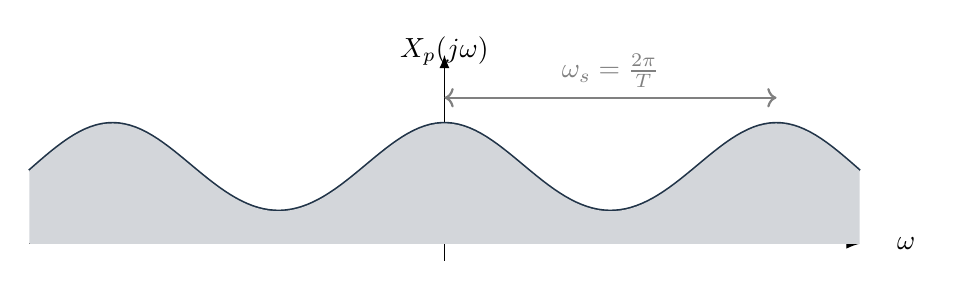
\begin{tikzpicture}
                \begin{axis}[
                    width=\textwidth, height=4.2cm,
                    axis lines=middle, axis line style={-{Latex}},
                    xmin=-10, xmax=10, ymin=-0.2, ymax=2.2,
                    xtick={0}, xticklabels={$0$},
                    ytick=\empty, xlabel={$\omega$}, ylabel={$X_p(j\omega)$}, clip=false,
                    xlabel style={anchor=west, xshift=10pt}, ylabel style={yshift=10pt, anchor=north},
                    declare function={
                            gauss(\x) = 1.4*exp(-(\x*\x)/8);
                            dtft(\x) = gauss(\x) + gauss(\x-8) + gauss(\x+8);
                        }
                    ]
                    \addplot[samples=150, domain=-10:10, very thick, PrimaryColor] {dtft(x)};
                    \addplot[fill=PrimaryColor!20, draw=none, domain=-10:10, samples=150] {dtft(x)} \closedcycle;
                    \draw[<->, thick, gray] (axis cs:0,1.7) -- node[above] {$\omega_s = \frac{2\pi}{T}$} (axis cs:8,1.7);
                \end{axis}
            \end{tikzpicture}

            \vspace{0.1cm}
            \textbf{Discrete Fourier Transform} \\ \smallskip
            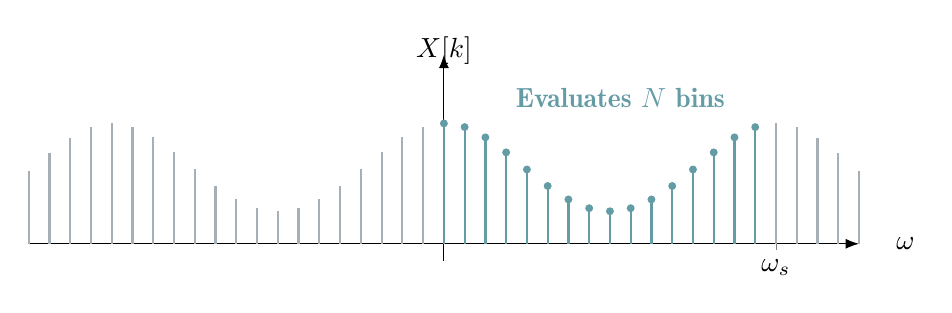
\begin{tikzpicture}
                \begin{axis}[
                    width=\textwidth, height=4.2cm,
                    axis lines=middle, axis line style={-{Latex}},
                    xmin=-10, xmax=10, ymin=-0.2, ymax=2.2,
                    xtick={0, 8}, xticklabels={$0$, $\omega_s$},
                    ytick=\empty, xlabel={$\omega$}, ylabel={$X[k]$}, clip=false,
                    xlabel style={anchor=west, xshift=10pt}, ylabel style={yshift=10pt, anchor=north},
                    declare function={
                            gauss(\x) = 1.4*exp(-(\x*\x)/8);
                            dtft(\x) = gauss(\x) + gauss(\x-8) + gauss(\x+8);
                        }
                    ]
                    \addplot[ycomb, mark=none, thick, PrimaryColor!40, samples=41, domain=-10:10] {dtft(x)};
                    \addplot[ycomb, mark=*, AccentColor, thick, samples=16, domain=0:7.5, mark size=1pt] {dtft(x)};
                    \node[AccentColor, font=\bfseries, anchor=west] at (axis cs:1.5, 1.7) {Evaluates $N$ bins};
                \end{axis}
            \end{tikzpicture}
        \end{column}
    \end{columns}
\end{frame}

\begin{frame}{Frequency Mapping of the DFT}
    \begin{columns}
        \begin{column}{0.42\textwidth}
            \begin{insightbox}{How to Read the DFT Bins}
                We compute from $0 \to \omega_s$, but physical signals are centered around $0$. Because the spectrum repeats (periodicity), we just "fold" the second half back!
                \vspace{0.2cm}
                \begin{itemize}
                    \item \textbf{First Half:} \textcolor{PrimaryColor}{\textbf{Positive} frequencies} ($0 \le k < N/2$).
                    \item \textbf{Second Half:} \textcolor{AccentColor}{\textbf{Negative} frequencies} ($N/2 < k < N$).
                \end{itemize}
            \end{insightbox}
        \end{column}

        \begin{column}{0.54\textwidth}
            \vspace*{0.3cm}
            \centering
            \textbf{DFT Bin Index Mapping} \\ \smallskip
            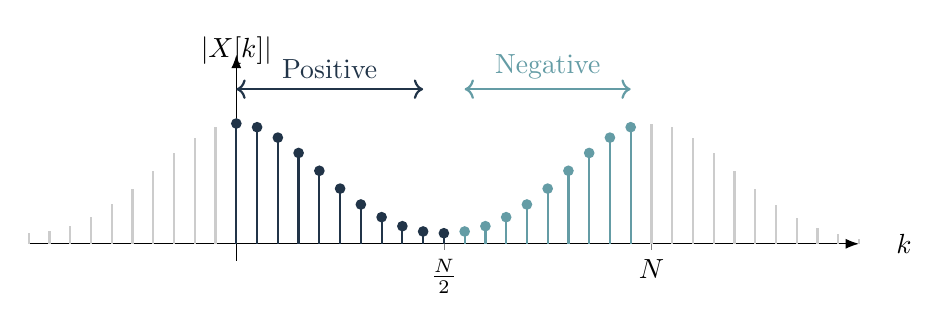
\begin{tikzpicture}
                \begin{axis}[
                    width=\textwidth, height=4.2cm,
                    axis lines=middle, axis line style={-{Latex}},
                    xmin=-5, xmax=15, ymin=-0.2, ymax=2.2,
                    xtick={0, 5, 10}, xticklabels={$0$, $\frac{N}{2}$, $N$},
                    ytick=\empty, xlabel={$k$}, ylabel={$|X[k]|$}, clip=false,
                    xlabel style={anchor=west, xshift=10pt}, ylabel style={yshift=10pt, anchor=north},
                    declare function={
                            gauss(\x) = 1.4*exp(-(\x*\x)/8);
                            dtft(\x) = gauss(\x) + gauss(\x-10) + gauss(\x+10);
                        }
                    ]
                    \addplot[ycomb, mark=none, thick, gray!40, samples=41, domain=-5:15] {dtft(x)};
                    \addplot[ycomb, mark=*, PrimaryColor, thick, samples=11, domain=0:5, mark size=1.5pt] {dtft(x)};
                    \addplot[ycomb, mark=*, AccentColor, thick, samples=9, domain=5.5:9.5, mark size=1.5pt] {dtft(x)};

                    \draw[<->, thick, PrimaryColor] (axis cs:0, 1.8) -- node[above] {Positive} (axis cs:4.5, 1.8);
                    \draw[<->, thick, AccentColor] (axis cs:5.5, 1.8) -- node[above] {Negative} (axis cs:9.5, 1.8);
                \end{axis}
            \end{tikzpicture}

            \vspace{0.1cm}
            \textbf{Equivalent Baseband Spectrum} \\ \smallskip
            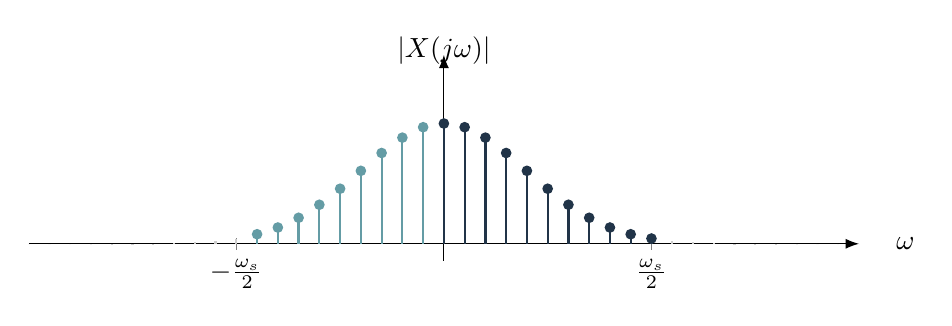
\begin{tikzpicture}
                \begin{axis}[
                    width=\textwidth, height=4.2cm,
                    axis lines=middle, axis line style={-{Latex}},
                    xmin=-10, xmax=10, ymin=-0.2, ymax=2.2,
                    xtick={-5, 0, 5}, xticklabels={$-\frac{\omega_s}{2}$, $0$, $\frac{\omega_s}{2}$},
                    ytick=\empty, xlabel={$\omega$}, ylabel={$|X(j\omega)|$}, clip=false,
                    xlabel style={anchor=west, xshift=10pt}, ylabel style={yshift=10pt, anchor=north},
                    declare function={
                            gauss(\x) = 1.4*exp(-(\x*\x)/8);
                        }
                    ]
                    \addplot[ycomb, mark=none, thick, gray!40, samples=41, domain=-10:10] {gauss(x)};
                    \addplot[ycomb, mark=*, PrimaryColor, thick, samples=11, domain=0:5, mark size=1.5pt] {gauss(x)};
                    \addplot[ycomb, mark=*, AccentColor, thick, samples=9, domain=-4.5:-0.5, mark size=1.5pt] {gauss(x)};
                \end{axis}
            \end{tikzpicture}
        \end{column}
    \end{columns}
\end{frame}

\begin{frame}{Rigorous Recovery (Periodic): 1. Continuous Spectrum}
    \begin{columns}
        \begin{column}{0.42\textwidth}
            \begin{insightbox}{Periodic Signals $\equiv$ Deltas}
                If our signal repeats perfectly forever with period $P$, it can be represented entirely by a Fourier Series!
                \begin{itemize}
                    \item Instead of a continuous smear, $X(j\omega)$ just becomes discrete \textbf{delta spikes} exactly at harmonics ($\omega_0$):
                \end{itemize}
                \vspace{-0.2cm}
                \begin{equation*}
                    X(j\omega) = 2\pi\sum_{m=-\infty}^{\infty} a_m \delta(\omega - m\omega_0)
                \end{equation*}
            \end{insightbox}
        \end{column}

        \begin{column}{0.54\textwidth}
            \vspace*{0.3cm}
            \centering
            \textbf{Time Domain: Periodic outside window} \\ \smallskip
            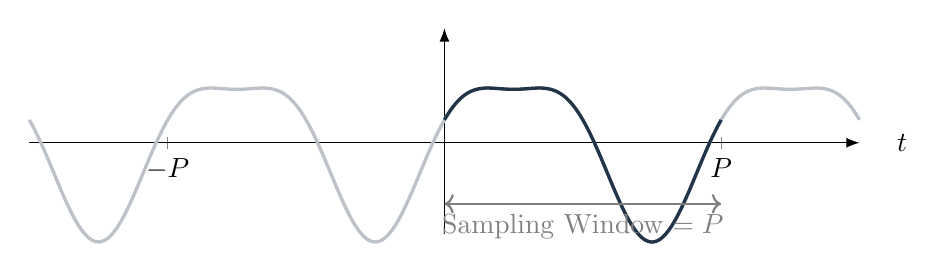
\begin{tikzpicture}
                \begin{axis}[
                    width=\textwidth, height=4.2cm,
                    axis lines=middle, axis line style={-{Latex}},
                    xmin=-15, xmax=15, ymin=-1.2, ymax=1.5,
                    xtick={-10, 0, 10}, xticklabels={$-P$, $0$, $P$},
                    ytick=\empty, xlabel={$t$}, clip=false,
                    xlabel style={anchor=west, xshift=10pt},
                    declare function={
                            wave(\x) = sin(deg(\x * 3.14159 / 5)) + 0.3*cos(deg(\x * 3.14159 / 2.5));
                        }
                    ]
                    \addplot[samples=200, domain=-15:15, very thick, PrimaryColor!30] {wave(x)};
                    \addplot[samples=100, domain=0:10, very thick, PrimaryColor] {wave(x)};
                    \draw[<->, thick, gray] (axis cs:0,-0.8) -- node[below] {Sampling Window $= P$} (axis cs:10,-0.8);
                \end{axis}
            \end{tikzpicture}

            \vspace{0.1cm}
            \textbf{Frequency Domain: Sum of Deltas $X(j\omega)$} \\ \smallskip
            \begin{tikzpicture}
                \begin{axis}[
                    width=\textwidth, height=4.2cm,
                    axis lines=middle, axis line style={-{Latex}},
                    xmin=-10, xmax=10, ymin=-0.2, ymax=2.2,
                    xtick={0, 2}, xticklabels={$0$, $\omega_0$},
                    ytick=\empty, xlabel={$\omega$}, ylabel={$X(j\omega)$}, clip=false,
                    xlabel style={anchor=west, xshift=10pt}, ylabel style={yshift=10pt, anchor=north},
                    declare function={gauss(\x) = 1.4*exp(-(\x*\x)/8);}
                    ]
                    \addplot[ycomb, mark=triangle*, thick, PrimaryColor, samples=7, domain=0:6, mark size=2pt] {gauss(x)};
                    \addplot[ycomb, mark=triangle*, thick, AccentColor, samples=6, domain=-6:-1, mark size=2pt] {gauss(x)};
                    \node[anchor=west] at (axis cs:6, 1.5) {Max freq $\omega_m$};
                    \draw[->, thick, gray] (axis cs:6, 1.4) -- (axis cs:6, 0.2);
                \end{axis}
            \end{tikzpicture}
        \end{column}
    \end{columns}
\end{frame}

\begin{frame}{Rigorous Recovery (Periodic): 2. Sampling (Nyquist)}
    \begin{columns}
        \begin{column}{0.42\textwidth}
            \begin{conceptbox}{Preserving the Spikes (Nyquist)}
                Remember, sampling creates infinite shifted copies of our delta spectrum!
                \vspace{-0.2cm}
                \begin{equation*}
                    X_p(j\omega) = \frac{1}{T}\sum_{r=-\infty}^{\infty} X(j(\omega-r\omega_s))
                \end{equation*}
                As long as we sample fast enough ($\omega_s > 2\omega_m$), we leave a clear gap. \textbf{Zero shifted copies overlap}, which implies exactly \textbf{zero aliasing}!
            \end{conceptbox}
        \end{column}

        \begin{column}{0.54\textwidth}
            \vspace*{0.3cm}
            \centering
            \textbf{Shifted Copies $X_p(j\omega)$ without Aliasing} \\ \smallskip
            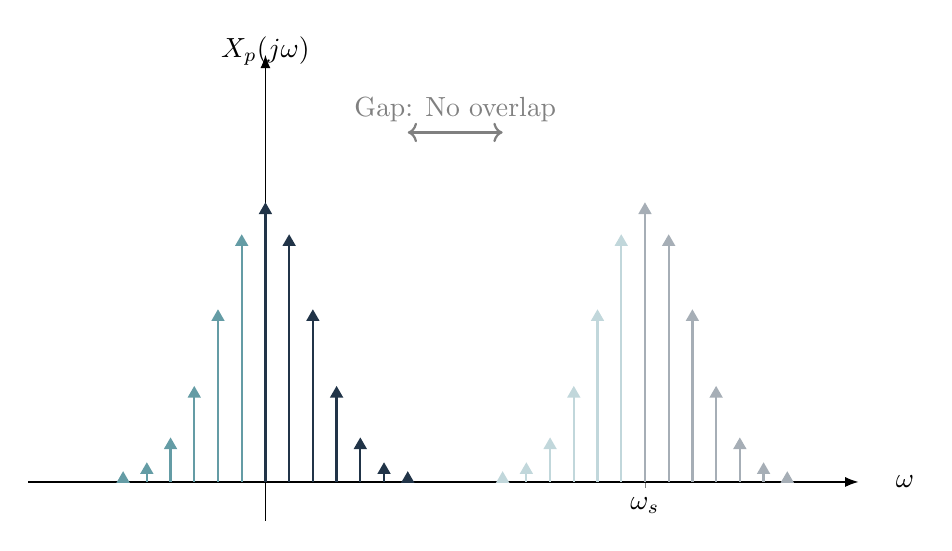
\begin{tikzpicture}
                \begin{axis}[
                    width=\textwidth, height=7.5cm,
                    axis lines=middle, axis line style={-{Latex}},
                    xmin=-10, xmax=25, ymin=-0.2, ymax=2.2,
                    xtick={0, 16}, xticklabels={$0$, $\omega_s$},
                    ytick=\empty, xlabel={$\omega$}, ylabel={$X_p(j\omega)$}, clip=false,
                    xlabel style={anchor=west, xshift=10pt}, ylabel style={yshift=10pt, anchor=north},
                    declare function={
                            gauss(\x) = 1.4*exp(-(\x*\x)/8);
                        }
                    ]
                    % Baseband
                    \addplot[ycomb, mark=triangle*, thick, PrimaryColor, samples=7, domain=0:6, mark size=2pt] {gauss(x)};
                    \addplot[ycomb, mark=triangle*, thick, AccentColor, samples=6, domain=-6:-1, mark size=2pt] {gauss(x)};

                    % Shifted r=1 copy
                    \addplot[ycomb, mark=triangle*, thick, PrimaryColor!40, samples=7, domain=16:22, mark size=2pt] {gauss(x-16)};
                    \addplot[ycomb, mark=triangle*, thick, AccentColor!40, samples=6, domain=10:15, mark size=2pt] {gauss(x-16)};

                    \draw[<->, thick, gray] (axis cs:6, 1.8) -- node[above] {Gap: No overlap} (axis cs:10, 1.8);
                \end{axis}
            \end{tikzpicture}
        \end{column}
    \end{columns}
\end{frame}

\begin{frame}{Rigorous Recovery (Periodic): 3. DFT Coefficient Isolation}
    \begin{columns}
        \begin{column}{0.42\textwidth}
            \begin{insightbox}{Perfect Isolation}
                By capturing exactly $N$ samples per period, our DFT evaluation bins \textbf{land perfectly} on top of our isolated deltas!
                \begin{itemize}
                    \item We perfectly extract the true $a_m$ amplitudes without any distortion!
                \end{itemize}
                \begin{equation*}
                    X[k] = X_p\left(j\frac{k\omega_s}{N}\right) \propto a_k
                \end{equation*}

                \footnotesize
                \textbf{\textcolor{PrimaryColor}{Positive $a_m$}}: Captured cleanly at the start bins.\\
                \textbf{\textcolor{AccentColor}{Negative $a_{-m}$}}: Captured reliably at the folded tail!
            \end{insightbox}
        \end{column}

        \begin{column}{0.54\textwidth}
            \vspace*{0.3cm}
            \centering
            \textbf{Discrete Fourier Transform Evaluates $X_p(j\omega)$} \\ \smallskip
            \begin{tikzpicture}
                \begin{axis}[
                    width=\textwidth, height=7.5cm,
                    axis lines=middle, axis line style={-{Latex}},
                    xmin=-2, xmax=18, ymin=-0.2, ymax=2.2,
                    xtick={0, 16}, xticklabels={$0$, $N$},
                    ytick=\empty, xlabel={$k$}, ylabel={$X[k]$}, clip=false,
                    xlabel style={anchor=west, xshift=10pt}, ylabel style={yshift=10pt, anchor=north},
                    declare function={
                            gauss(\x) = 1.4*exp(-(\x*\x)/8);
                            dtft(\x) = gauss(\x) + gauss(\x-16) + gauss(\x+16);
                        }
                    ]
                    \addplot[ycomb, mark=none, thick, gray!30, samples=17, domain=0:16] {dtft(x)};

                    \addplot[ycomb, mark=*, thick, PrimaryColor, samples=7, domain=0:6, mark size=2pt] {dtft(x)};
                    \addplot[ycomb, mark=*, thick, AccentColor, samples=6, domain=10:15, mark size=2pt] {dtft(x)};

                    \node[anchor=west, PrimaryColor, font=\bfseries] at (axis cs:1, 1.8) {Positive $+a_m$};
                    \node[anchor=west, AccentColor, font=\bfseries] at (axis cs:9.5, 1.8) {Negative $-a_m$};
                \end{axis}
            \end{tikzpicture}
        \end{column}
    \end{columns}
\end{frame}

\end{document}
